%TCIDATA{LaTeXparent=0,0,relatorio.tex}
                      

\chapter{Modelagem fuzzy Takagi-Sugeno de sistemas não lineares}\label{cap_ModelagemSisNaoLinearesporFuzzyTS}

\section{Introdução}

Sistemas dinâmicos não lineares variantes no tempo modelam boa parte dos problemas encontrados nas mais diversas áreas da engenharia \cite{bookogata:2003}. A observação do comportamento deste tipo de sistema, dado uma condição inicial, permite análises qualitativas da estabilidade destes \cite{bookkhalil:2003}. Quantitativamente, porém, a determinação da região de estabilidade e a aplicação de técnicas de controle para este tipo de sistema não são triviais, justamente devido à natureza não linear que possuem. Assim, métodos matemáticos são utilizados  a fim de ser obter modelos lineares equivalentes a estes sistemas, os quais facilitem o uso de ferramentas existentes na literatura. Neste contexto, este capítulo, além de apresentar uma discussão sobre sistemas não lineares,  discorre também sobre o uso do retrato de fase como um meio de analisar qualitativamente o comportamento de sistemas não lineares e aborda a utilização de lógica fuzzy, segundo a proposto por Takagi e Sugeno \cite{articlets:1985},  para a modelagem local de sistemas não lineares.

\section{Análise qualitativa de sistemas não lineares} \label{Sist-nao-lin-retrato-fase}

Um sistema é dito não linear quando a ele não é  possível aplicar o princípio da superposição, ou seja, a resposta a duas entradas distintas não pode ser calculada tratando uma resposta por vez e depois somando os resultados \cite{bookogata:2003}. Mesmo com a enorme gama de sistemas físicos representados como dinâmica linear, a grande maioria destes possui dinâmica real não linear, por isso o estudo de sistemas desta natureza torna-se praticamente inevitável do ponto de vista da engenharia.

\subsection{Sistemas não lineares}

Sistemas não lineares podem ser descritos como o conjunto formado por um número finito de equações ordinárias diferenciais de primeira ordem na forma
\begin{equation}\label{sist_nao_linear_generico}
\mathbf{\dot{x}}=g\mathbf{(x,u)}
\end{equation}
onde $x \in \rm I\!R^n$ é o vetor de estados, $u \in \rm I\!R^n$ o vetor dos sinais de entrada. Estes sistemas podem ser representados na forma
\begin{equation}\label{eq:noninear_system}
\mathbf{\dot{x}} = \mathbf{A(x)x} + \mathbf{B(x)u}
\end{equation}
sendo $A(x) \in\rm I\!R^{n \times n}$ e $B(x) \in \rm I\!R^{n \times m}$ matrizes cujos elementos podem depender dos estados do sistema e os quais também são funções contínuas num certo domínio de interesse. Este tipo de representação pode ser não único, ou seja, podem ser escolhidos diferentes $\textbf{A(x)}$ e $\textbf{B(x)}$ a partir da mesma função $g\textbf{(x,u)}$, estas diferentes escolhas são feitas pelo projetista. A seguir é mostrado um exemplo de um sistema não linear $g(\textbf{x,u})$ para o qual se obtém mais de uma representação diferente para $\textbf{A(x)}$ e $\textbf{B(x)}$.

\begin{example}[Representações distintas de um mesmo sistema não linear] Considere o sistema não linear dado por
	\begin{equation*}
		g(\textbf{x,u}) = x_1^2x_2+u
	\end{equation*}
	Este sistema pode ser representado como
	\begin{equation*}
	\dot{\textbf{x}} = a(\textbf{x})x_2+b(\textbf{x})u,\quad a(\textbf{x}) = x_1^2,\quad b(\textbf{x}) = 1
	\end{equation*}
	De forma análoga, o sistema pode ser representado como
	\begin{equation*}
	\dot{\textbf{x}} = a(\textbf{x})x_1+b(\textbf{x})u,\quad a(\textbf{x}) = x_1x_2,\quad b(\textbf{x}) = 1
	\end{equation*}
	Desta maneira, é possível verificar que um mesmo sistema não linear pode ser representado de diferentes formas, que dependerão da escolha do projetista.
	\label{ex:nonlinear_system_multiple_representation}
\end{example}

Como em (\ref{eq:noninear_system}) o sistema não depende explicitamente do tempo, este é dito como um sistema autônomo invariante no tempo \cite{bookkhalil:2003}. Nos exemplos apresentados neste trabalho, o sinal de entrada $u$ não será explicitado, utilizando-se, assim, equações de estado não forçadas \cite{bookkhalil:2003}. Trabalhar com este tipo de equação de estado não necessariamente significa que a entrada é nula, mas pode ser que a entrada tenha sido especificada como uma função dependente do tempo, ou das variáveis de estado, ou de ambos, de forma que se elimine $u$, obtendo uma equação de estados não forçada. Assim, neste trabalho estaremos interessados na classe particular de sistemas não lineares descritos na forma
\begin{equation}\label{eq:nonlinear_system_f_x}
\dot{\textbf{x}} = f(\textbf{x})
\end{equation}
Que pode ser representada equivalentemente por
\begin{equation}\label{eq:nonlinear_system_mean_representation}
	f(\textbf{x})=\textbf{A}(\textbf{x})\textbf{x}
\end{equation}
Para os sistemas apresentados no decorrer deste trabalho, quando as equações de estado apresentarem sinal de entrada, este será definido como um sinal de valor constante fixo $\textbf{u}(t)=\textbf{u}^*$ para qualquer instante de tempo $t \geq 0$, de forma tal que sejam feitas manipulações matemáticas a fim de se obter o sistema na forma (\ref{eq:nonlinear_system_mean_representation}).

\subsection{Pontos de equilíbrio}\label{subsec_pontoEq}

A engenharia de controle tem como um dos principais desafios manter o sistema funcionando em uma faixa de operação denominada regime permanente. Um sistema opera em regime permanente quando as variáveis de estado se mantêm constantes a medida que o tempo passa. Estes valores constantes correspondem ao ponto de equilíbrio do sistema\cite{bookboydl:1994}. Assim, o comportamento de sistemas modelados por equações de estado, como o da equação \ref{eq:noninear_system}, é caracterizado quanto aos seus  pontos de equilíbrio.

Ponto de equilíbrio, segundo (Khalil, 2003)\cite{bookkhalil:2003}, é definido como um ponto $\mathbf{x = x^*}$ no espaço de estados tal que, seja qual for o ponto inicial $\mathbf{x_0}$ em relação a $\mathbf{x^*}$, o sistema sempre convergirá para $\mathbf{x^*}$, para qualquer instante de tempo futuro.
Os pontos de equilíbrio da equação (\ref{eq:nonlinear_system_f_x}) equivalem às suas raízes reais, tais que
\begin{equation}\label{eq:ponto_de_eq}
\mathbf{f(x)} = 0.
\end{equation}

Caso a equação \ref{eq:ponto_de_eq} possua mais de uma raiz real, pode-se definir uma vizinhança local para cada ponto de equilíbrio. Desta forma, se houver apenas um ponto de equilíbrio na vizinhança, diz-se que este é um ponto de equilíbrio isolado. Caso contrário, diz-se que a vizinhança possui uma continuidade de pontos de equilíbrio.

Por convenção, será assumido que o sistema (\ref{eq:nonlinear_system_f_x}) possui um único ponto de equilíbrio na região de interesse no plano de estados e este ponto sempre estará localizado na origem, sem perdas de generalidade, utilizando-se do artifício de mudança de variáveis, conforme descrito a seguir.

Suponha que o ponto de equilíbrio do sistema (\ref{eq:nonlinear_system_f_x}) seja $\textbf{x = x}^*$, tal que $\textbf{x}^* \neq \textbf{0}$. E considere a mudança de variáveis $\textbf{y = x - x}^*$. A derivada de $\textbf{y}$ é dada por
\begin{equation*}\mathbf{\dot{y} = \dot{x} = f(x) = f(y + x^*)}
 \myeq 
g(\textbf{y})
\end{equation*}
onde $g(\textbf{0}) = \textbf{0}$. Portanto, na nova variável $\textbf{y}$, o sistema tem ponto de equilíbrio na origem, sem que haja perda de generalidade.

\subsection{Retrato de fase} \label{subsec_phasePortrait}

Considerando o caso específico em que o sistema da equação (\ref{eq:nonlinear_system_f_x}) possui apenas duas variáveis de estado, ou seja, para sistemas de segunda ordem, é possível representar a curva de respostas destes em um plano. Assim, pode-se fazer uma análise qualitativa do comportamento do sistema, gerando-se a curva de resposta para $x_1$ e $x_2$ para instantes de tempo maiores que zero sobre o plano x1-x2, denominado plano de estados. As curvas de resposta são traçadas pela combinação de vetores tangenciais à resposta do sistema a partir de um dado ponto inicial $\mathbf{x_0}$.

Um mesmo sistema pode apresentar inúmeras curvas de resposta diferentes, cada uma oriunda de um ponto inicial $\mathbf{x_0}$ distinto. Para se obter uma representação mais próxima do comportamento real da curva de resposta de $\mathbf{f(x)}$ a partir de $\mathbf{x_0}$, fixam-se os módulos dos vetores tangenciais às respostas em um valor específico, conservando a direção e o sentido destes, de forma que sejam traçados vetores equidistantes sobre o plano de estados, até que se obtenha a curva de resposta.

A representação de todas as curvas de resposta sobre uma determinada região no plano de estados constitui o\textbf{ retrato de fase} do sistema\cite{bookkhalil:2003}. Desta maneira, o retrato de fase é obtido percorrendo-se o grid do plano x1-x2, de forma que, $\mathbf{x_0}$ será um novo ponto em x1-x2 para cada posição do grid e a trajetória da resposta é obtida para cada $\mathbf{x_0}$ distinto. A figura do retrato de fase do sistema permite apenas uma análise qualitativa deste, visto que, uma vez que o tempo é omitido ao se plotar as trajetórias, torna-se inviável obter a resposta $\mathbf{x(t)}$ associada a uma trajetória \cite{bookkhalil:2003}.

A análise qualitativa que se pode fazer a partir do retrato de fase está relacionada com a estabilidade dos pontos de equilíbrio do sistema. Portanto, faz-se importante escolher uma região do plano de estados tal que contenha todos, ou a maioria, destes pontos de equilíbrio.

Um ponto de equilíbrio será estável quando qualquer resposta iniciada próxima a este se mantém sempre próxima; e é instável, caso se afaste. A Figura \ref{fig:pontos_eq_retrato_fase}, ilustra exemplos de retrato de fase em torno de um ponto de equilíbrio estável e outro instável, onde o ponto de equilíbrio é representado na cor vermelha e as trajetórias de resposta que geram o retrato de fase em azul.

\begin{figure}[htbp]
	\centering
	\subfigure[ref1][Ponto de equilíbrio estável]{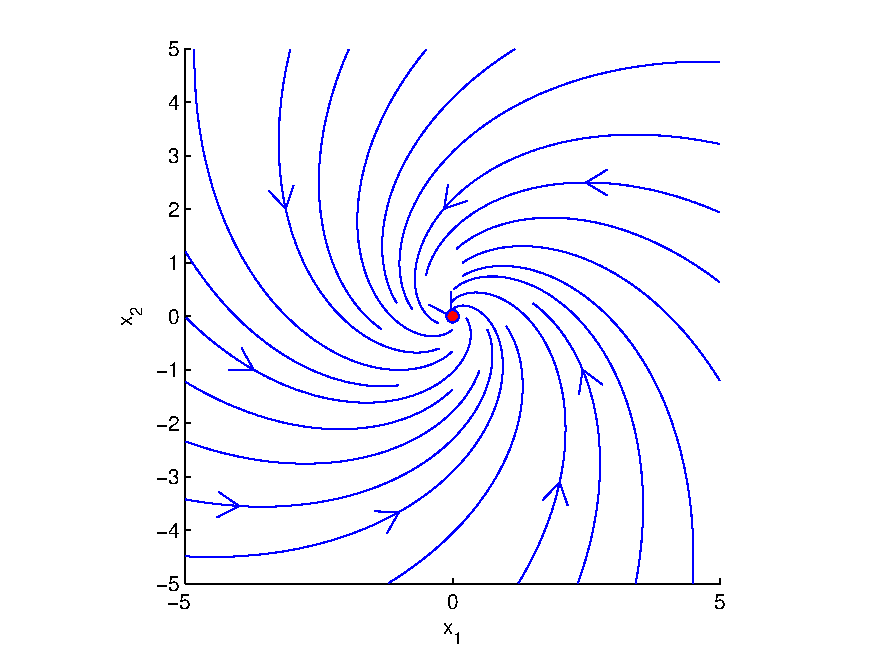
\includegraphics[width=7cm]{phase_portrait_stable}}
	\qquad
	\subfigure[ref2][Ponto de equilíbrio instável]{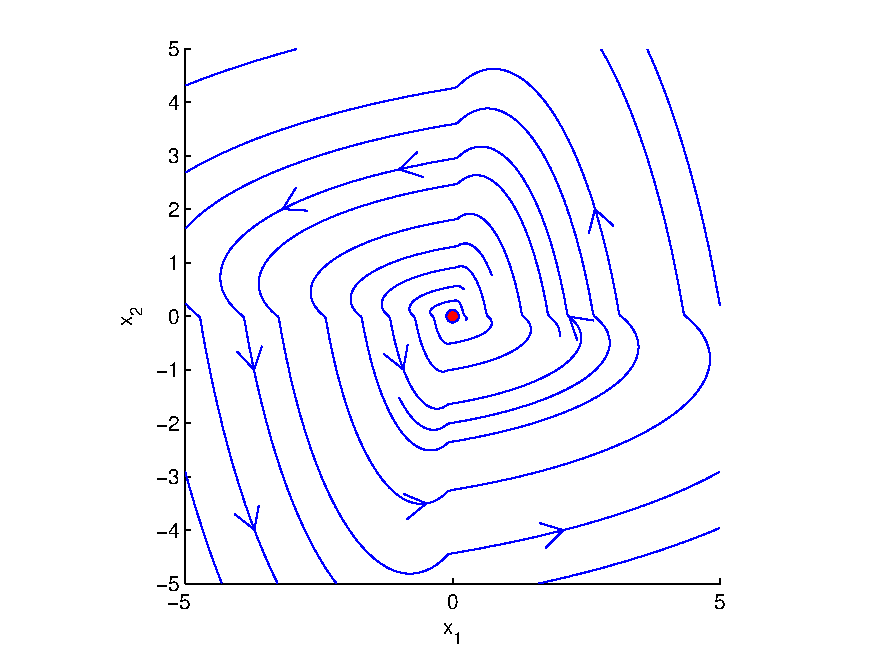
\includegraphics[width=7cm]{phase_portrait_unstable}}
	\caption{Retrato de fase para pontos de equilíbrio estável e instável}
	\label{fig:pontos_eq_retrato_fase}
\end{figure}

Além de estável e instável, o retrato de fase pode revelar outras configurações para os pontos de equilíbrio, como são os casos apresentados na Figura \ref{fig:outras_config_retrato_fase}, por exemplo.
No caso em que as trajetórias, além de se manter próximas ao ponto de equilíbrio, também convirjam a este quando o tempo tende ao infinito, o ponto de equilíbrio é dito como assintoticamente estável, como mostra a Figura \ref{fig:outras_config_retrato_fase} (a).
Já a Figura \ref{fig:outras_config_retrato_fase} (b) ilustra o caso em que as trajetórias se aproximam do ponto de equilíbrio a partir de determinados pontos iniciais e em seguida se afastam, mas sem nunca atingirem o ponto de equilíbrio. Este tipo de comportamento caracteriza o ponto de equilíbrio como um ponto de sela. 

\begin{figure}[htbp]
	\centering
	\subfigure[ref1][Ponto de equilíbrio  assintoticamente estável]{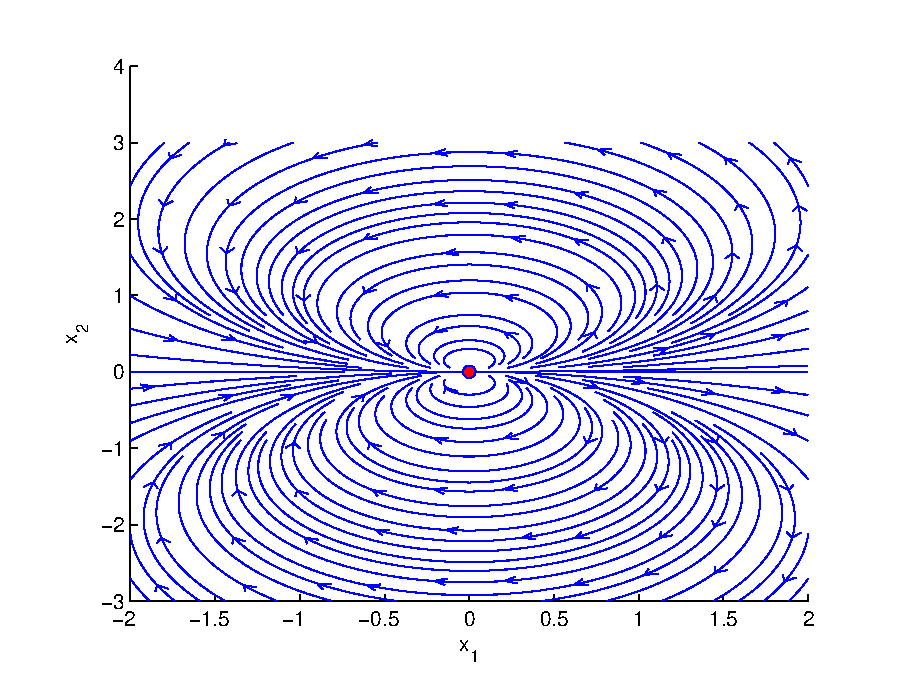
\includegraphics[width=7cm]{phase_portrait_assimptotically_stable}}
	\qquad
	\subfigure[ref2][Ponto de equilíbrio como ponto de sela]{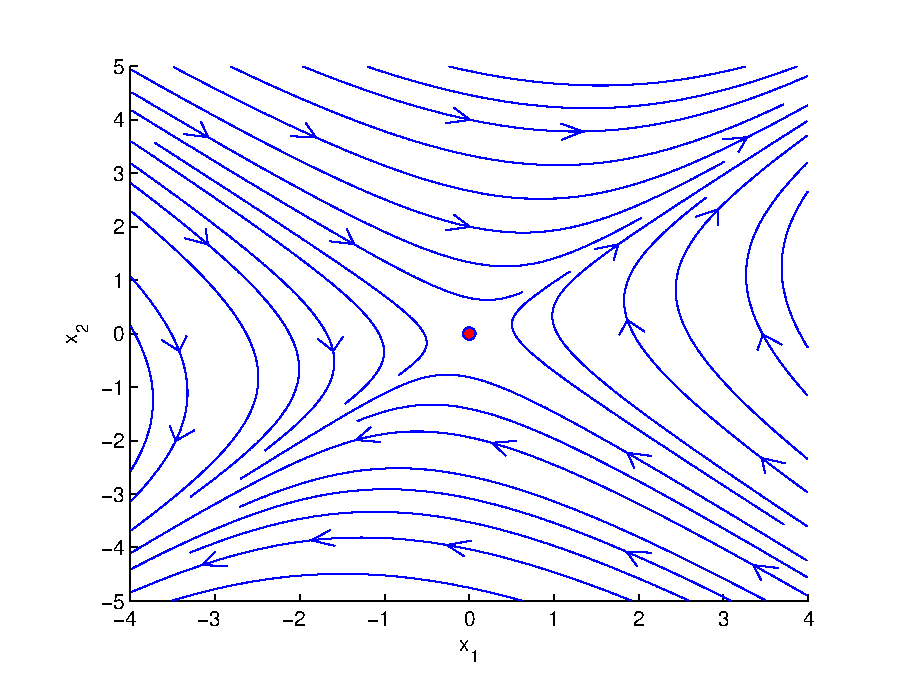
\includegraphics[width=7cm]{phase_portrait_saddle}}
	\caption{Retrato de fase para pontos de equilíbrio  assintoticamente estável e ponto de sela}
	\label{fig:outras_config_retrato_fase}
\end{figure}

Para o caso em que se tem um sistema de terceira ordem, cujo sistema não linear possui três variáveis de estado, também é possível obter o retrato de fase. O plano de estados passa a ser tridimensional e cada ponto terá três componentes: $\mathbf{x_1}$, $\mathbf{x_2}$ e $\mathbf{x_3}$. A partir daí a ideia passa a ser a mesma descrita para sistemas de segunda ordem.

Os próximos capítulos abordarão métodos de verificação de estabilidade de sistemas não lineares e a obtenção da região em que a estabilidade é garantida. Assim, será possível utilizar o retrato de fase como um meio de validar a região de estabilidade, visto que o retrato de fase é uma aproximação bastante realista do comportamento do sistema ao longo do tempo para diversos pontos iniciais \cite{bookkhalil:2003}.

\subsection{Exemplos} \label{subsection:descr_exemplos}

Nesta seção serão apresentados os exemplos utilizados nas análises e validações dos tópicos discutidos no decorrer deste trabalho. O primeiro exemplo consiste em um sistema não linear de segunda ordem retirado do artigo publicado por Lee, Park an Joo em 2011\cite{article:LPJ:2011}. Em seguida, tem-se um sistema de terceira ordem, que equivale ao modelo de um inversor de tensão conectado a um barramento de corrente alternada infinito. Por fim, o terceiro exemplo apresentado, um sistema  de quarta ordem, corresponde ao modelo do processo  de quatro tanques não linear disponibilizado nas instalações do Laboratório de Automação e Robótica da Universidade de Brasília (LARA - UnB).

\begin{example}
[Sistema não linear de segunda ordem \cite{article:LPJ:2011}] Considere o sistema não linear de segunda ordem descrito por
\begin{equation*}
\mathbf{ \begin{bmatrix}\dot{x_1}\\ \dot{x_2} \end{bmatrix} = \begin{bmatrix} -2 & 4\\  -1 - \dfrac{\lambda (1 - sen(x_1))}{2} & -2 \end{bmatrix} \begin{bmatrix}x_1 \\ x_2 \end{bmatrix}}
\end{equation*}
onde $\lambda$ é um escalar e $\mathbf{C_1 = \{x(t) \in \rm I\!R^n | |x_i(t)| \leq \pi/2, i \in \{1,2\}\}}$. Inicialmente, será assumido que $\lambda = 20$.
\label{example_LPJ12}
\end{example}

Para se obter o retrato de fase deste sistema, primeiramente deve-se encontrar os pontos de equilíbrio, que correspondem à solução do sistema para $\dot{x}_1$ = 0 e $\dot{x}_2$ = 0. Neste caso, verifica-se que o sistema possui um único ponto de equilíbrio\footnote{para obter os pontos de equilíbrio utilizou-se a função \textit{fsolve} do Matlab, que retorna o vetor \textbf{x} correspondente à solução da equação \textbf{f(x) = 0}.}$^,$\footnote{$x^*\triangleq x(0)$} dado por
\begin{equation*}
\mathbf{
\begin{bmatrix}x^*_1\\x^*_2\end{bmatrix} = \begin{bmatrix}0\\0\end{bmatrix}}
\end{equation*}

O retrato de fase do sistema corresponde às trajetórias obtidas assumindo-se diferentes pontos iniciais sobre do plano de estados limitado pela região contida no domínio de ${x_1}$ e ${x_2}$ e é apresentado na Figura \ref{fig:retrato_fase_ex2_LPJ12}.

\begin{figure}[htbp]
	\centering
	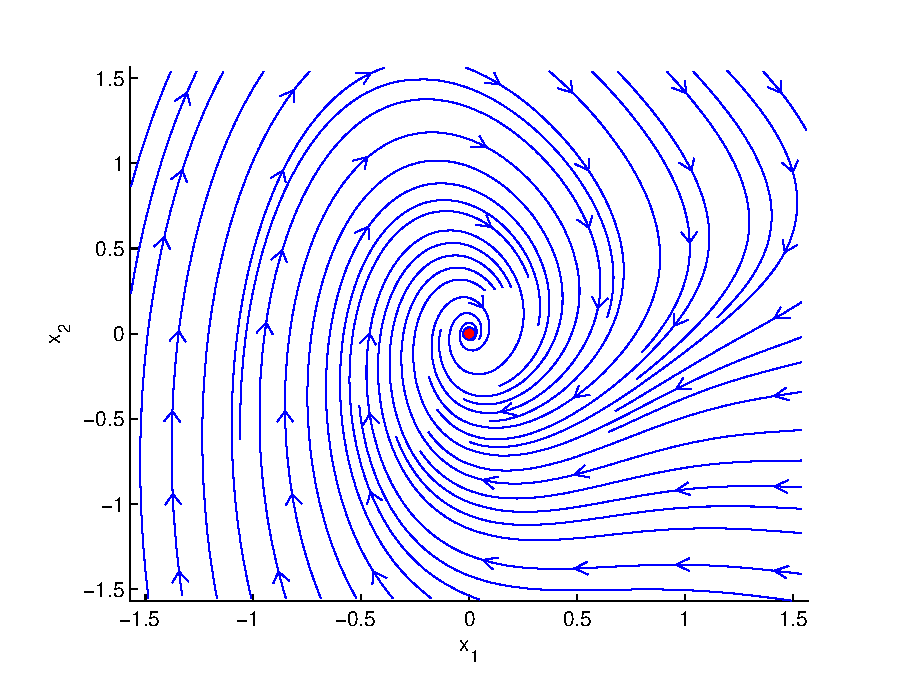
\includegraphics[width=10cm]{phase_portrait_ex2_LPJ12}
	\caption{Retrato de fase do sistema de segunda ordem do Exemplo \ref{example_LPJ12}. As trajetórias das respostas para os diferentes pontos iniciais estão representadas em azul e o ponto de equilíbrio aparece em vermelho.}
	 \label{fig:retrato_fase_ex2_LPJ12}
\end{figure}

O retrato de fase apresentado na Figura \ref{fig:retrato_fase_ex2_LPJ12} evidencia que o ponto de equilíbrio do sistema é assintoticamente estável, uma vez que todas as trajetórias de resposta para diferentes pontos iniciais dentro do domínio de \textbf{x} são atraídas para o ponto de equilíbrio.

\begin{example} [Sistema \textit{Droop}] O sistema proposto neste exemplo baseia-se no problema de controle de frequência e potência ativa para sistemas, que é definido pela dependência existente entre essas duas grandezas. A alteração da frequência afeta diretamente a potência ativa do sistema, Assim, reguladores de velocidade, ou de inclinação, são utilizados para prover o devido carregamento de sistemas interconectados.

Neste contexto, assuma um inversor de tensão de módulo $E_i$ e fase $\delta_i$ conectado a um barramento CA infinito com tensão de módulo $E_o$ e fase $0^{\circ}$ através de uma impedância de saída com módulo $Z_{oi}$ e fase $\theta_i$, conforme mostra a Figura \ref{fig:inversor_CA}.

\begin{figure}[htbp]
	\centering
	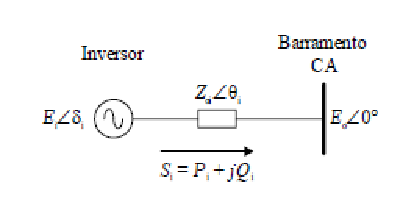
\includegraphics[width=6cm]{barramento}
	\caption{Inversor conectado a um barramento CA infinito}
	 \label{fig:inversor_CA}
\end{figure}

A potência aparente entregue pelo inversor ao barramento infinito, na forma retangular, é dada por
\begin{equation}
S_i = E_o(\dfrac{E_i\cos(\delta_i)-E_o+jE_i\sin(\delta_i)}{Z_{oi}\cos(\theta_i)+jZ_{oi}\sin(\theta_i)}).
\end{equation}
Separando-se  a parte real e a parte imaginária, definem-se as contribuições de potência ativa e reativa do inversor para o barramento CA, tal que
\begin{equation}\label{P_ativ}
P_i = (\dfrac{E_iE_o}{Z_{oi}}\cos(\delta_i)- \dfrac{E_o^2}{Z_{oi}})\cos(\theta_i)+\dfrac{E_iE_o}{Z_{oi}}\sin(\delta_i)\sin(\theta_i),
\end{equation}
\begin{equation}\label{P_reativ}
Q_i = (\dfrac{E_iE_o}{Z_{oi}}\cos(\delta_i)- \dfrac{E_o^2}{Z_{oi}})\sin(\theta_i)+\dfrac{E_iE_o}{Z_{oi}}\sin(\delta_i)\cos(\theta_i).
\end{equation}\label{P_i}
Quando a impedância de saída do inversor é resistiva, de modo que $\theta_i = 0$ e $Z_{oi} = R_{oi}$, então as expressões \ref{P_ativ} e \ref{P_reativ} podem ser rescritas como
\begin{equation}
P_i = \dfrac{E_iE_o\cos(\delta_i)- E_o^2}{R_{oi}},
\end{equation}
\begin{equation}\label{Q_i}
Q_i = -\dfrac{E_iE_o\sin(\delta_i)}{R_{oi}}.
\end{equation}
Considerando um ângulo de defasagem muito pequeno ($\delta_i \simeq 0$), as equações \ref{P_i} e \ref{Q_i} podem ser simplificadas considerando-se $\sin(\delta_i)\simeq\delta_i$ e $\cos(\delta_i)\simeq 1$.
\begin{equation}
P_i = \dfrac{E_iE_o- E_o^2}{R_{oi}},
\end{equation}
\begin{equation}
Q_i = -\dfrac{E_iE_o\delta_i}{R_{oi}}.
\end{equation}
Além disso, assumindo-se $Pi\sim E_i$ e $Q_i\sim -\delta_i$, tem-se as leis de controle do método \textit{Droop} convencional para a impedância de saída resistiva dadas por
\begin{equation}
E_i = E^*-n_i(P_i-P_i^*),
\end{equation}
\begin{equation}\label{lei_contr}
\omega_i = \omega^* + m_i(Q_i - Q^*).
\end{equation}
onde $E^*$ é a tensão de referência, $\omega^*$ é a frequência angular de referência, $P_i^*$ é a potência ativa de referência e $Q_i^*$ é a potência reativa de referência.

O coeficiente $n_i$ é geralmente determinado pela variação de tensão desejada para uma determinada variação de potência ativa, conforme a expressão
\begin{equation}
n_i = \dfrac{\Delta E_i}{\Delta P_i}.
\end{equation}
De modo semelhante, o coeficiente $m_i$ é determinado pela variação de frequência desejada para uma determinada variação de potência reativa, de acordo com a equação
\begin{equation}
m_i = \dfrac{\Delta \omega_i}{\Delta Q_i}.
\end{equation}
Assumindo, então, que os algoritmos de cálculo de $P_i$ e $Q_i$ possam ser modelados por um filtro passa-baixas de primeira ordem, tem-se
\begin{equation}
P_{f_i} = \dfrac{\omega_{pb}}{s+\omega_{pb}}P_i,
\end{equation}
\begin{equation}
Q_{f_i} = \dfrac{\omega_{pb}}{s+\omega_{pb}}Q_i.
\end{equation}
Equações tais que equivalem a
\begin{equation}
\dfrac{dP_{f_i}}{dt} = -\omega_{pb}P_{f_i}+\omega_{pb}P_i,
\end{equation}
\begin{equation}
\dfrac{dQ_{f_i}}{dt} = -\omega_{pb}Q_{f_i}+\omega_{pb}Q_i.
\end{equation}
Sabendo ainda que o ãngulo $\delta_i$ é obtido integrando-se a frequência $\omega_i$ a partir da lei de controle \ref{lei_contr}, pode-se escrever
\begin{equation}
\dfrac{d\delta_i}{dt} = m_i(Q_{f_i} - Q_i^*).
\end{equation}

Inibindo-se o termo subscrito $i$ das variáveis, considerando-se $\omega_{pb} = \omega_f$ e assumindo $Q_i^* = Q_{ref}$, $E_i^* = E_{ref}$ e $P_i^* = P_{ref}$, o modelo do sistema é obtido conforme segue.
\begin{equation} \label{eq:sist_droop}
\begin{cases}\dot{P}_f = -\omega_f P_f+\dfrac{\omega_f(V(E_{ref}-n(P_f-P_{ref}))\cos(\delta)-V^2)}{R_o}\\
\dot{Q}_f=
-\omega_f Q_f-
\dfrac{\omega_f V(E_{ref}-n(P_f - P_{ref}))\sin(\delta)}
{R_o}\\
\dot{\delta}=m(Qf-Q_{ref})\end{cases}
\end{equation}
Onde, $\omega_ f = 2\cdot\pi\cdot60 \dfrac{rad}{s}$, 
$V = 311 V$, 
$E_{ref} = 311 V$, 
$m = \dfrac{3.77}{22000} \dfrac{m}{s VAR}$, 
$n = \dfrac{20}{22000} \dfrac{m}{s W}$, 
$R_o = 0.1 \Omega$, 
$P_{ref} = 22000 W$ e 
$Q_{ref} = 0 VAR$.

As variáveis de estado são limitadas, tais que $C = \{x(t) \in \rm I\!R^3 | x_1(t) = P_f \in [0; 25000], x_2(t) = Q_f \in [-70000; 5000], x_3(t) = \delta \in [-0.02; 0.1]\}$.
\end{example}\label{ex:droop_UFSM}

Para se obter os pontos de equilíbrio do sistema, faz-se $\dot{\textbf{x}}(t) = 0$. Desta maneira, tem-se os pontos de equilíbrio
\begin{equation*}
\begin{bmatrix}x^*_1\\x^*_2\\x^*_3\end{bmatrix} = \begin{bmatrix}1.6252e+04\\0\\N*\pi\end{bmatrix}
\end{equation*}
em que $N = 0, 1, 3, ... 5$. Porém, dado que a variável de estado $x_3(t) = \delta$ é limitada no intervalo $[-0.02; 0.1]$, o único valor de $N$ que satisfaz esta limitação é $N = 0$. Assim, o ponto de equilíbrio do sistema a ser considerado é $\textbf{x}^* = \begin{bmatrix}1.6252e+04&0&0\end{bmatrix}'$.

Escolhendo-se arbitrariamente o ponto inicial $x_{inicial} = \begin{bmatrix}10000&1000&0.01\end{bmatrix}'$, obtemos a trajetória da resposta do sistema a partir deste ponto, conforme mostra a Figura \ref{fig:resp_droop}

\begin{figure}[htbp]
	\centering
	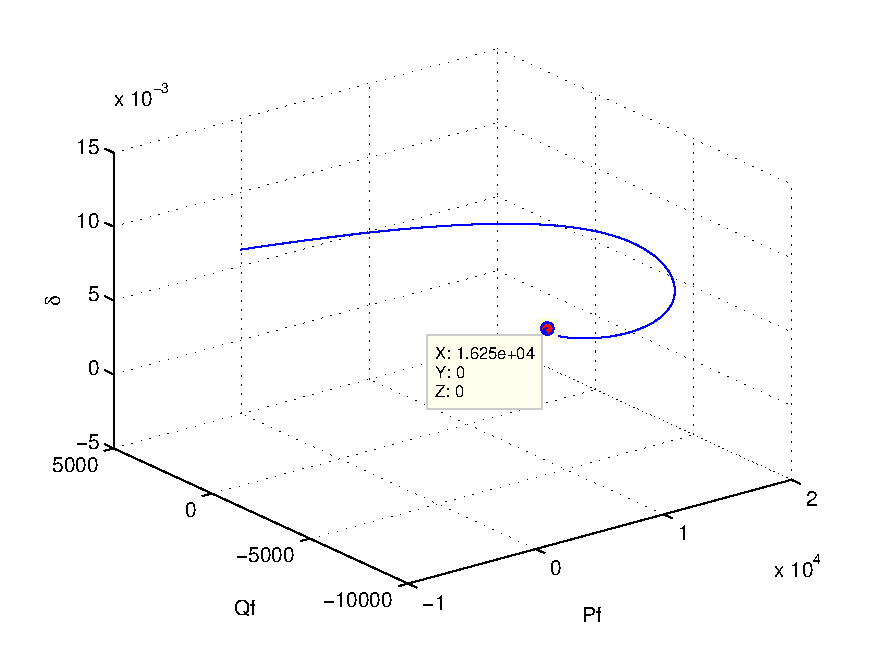
\includegraphics[width=10cm]{droop_answer_to_arbitrary_initial_value}
	\caption{Trajetória da resposta do sistema droop para o ponto inicial $x_{inicial} = [10000\quad1000\quad0.01]'$. A curva em azul corresponde à trajetória da resposta, enquanto o ponto em vermelho equivale ao ponto de equilíbrio do sistema}
	 \label{fig:resp_droop}
\end{figure}

Para este ponto inicial, é possível notar que a trajetória converge para o ponto de equilíbrio, sendo este um ponto de equilíbrio estável.

Ao se varrer um conjunto de pontos iniciais dentro da região representada pelos limites das variáveis de estado, é possível obter as  trajetórias de resposta do sistema a partir de cada ponto inicial. A Figura \ref{fig:droop_trajetorias} mostra estas trajetórias obtidas da varredura desta região para diferentes pontos iniciais.

\begin{figure}[htbp]
	\centering
	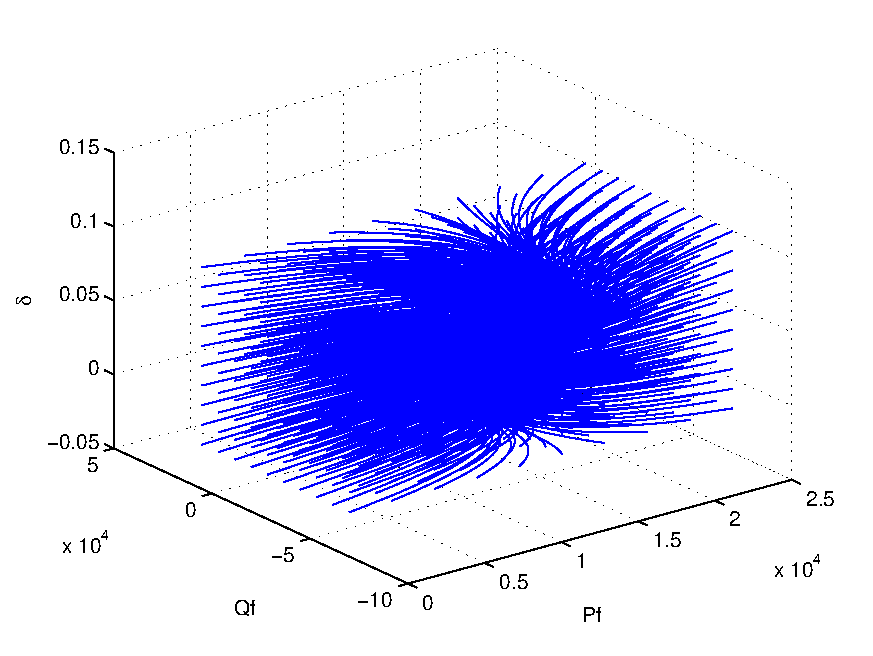
\includegraphics[width=10cm]{droop_answers_trajectories}
	\caption{Trajetórias de respostas do sistema para diferentes pontos iniciais definidos dentro da região contida pelos limites das variáveis de estado}
	 \label{fig:droop_trajetorias}
\end{figure}

Embora não seja claro enxergar na Figura \ref{fig:droop_trajetorias}, a simulação realizada para gerar esta imagem permitiu comprovar que todas as trajetórias obtidas a partir da variação dos pontos iniciais convergiram para o ponto de equilíbrio, constatando-se, de fato, que o ponto de equilíbrio  do sistema na região limitada pelas restrições das variáveis de estado é um ponto de equilíbrio estável.

Como neste trabalho se trabalhará com sistemas cujo ponto de equilíbrio encontra-se na origem, será utilizada mudança de variável $\mathbf{x_d = x - x^*}$ para deslocar o ponto de equilíbrio $\textbf{x}^* = \begin{bmatrix}1.6252e+04&0&0\end{bmatrix}'$ para a origem, tal que $\textbf{x}_d^* = \begin{bmatrix}0&0&0\end{bmatrix}'$ seja o ponto de equilíbrio deslocado do sistema, sem que haja perda de generalidade.

Assim, as variáveis de desvio serão
\begin{equation*}
\begin{bmatrix}x_{d_1}\\x _{d_2}\\x_{d_3}\end{bmatrix} = \begin{bmatrix}x_1\\x_2\\x_3\end{bmatrix} - \begin{bmatrix}x_1^*\\x_2^*\\x_3^*\end{bmatrix}
\end{equation*}

Assim, os novos limites das variáveis de estados são representados pela região poliédrica $C_1 = \{x_d(t) \in \rm I\!R^3 | x_{d1}(t) = P_f - x_1^* \in [-1.6252e+04; 25000 - 1.6252e+04], x_{d2}(t) = Q_f - x_2^* = Q_f \in [-70000; 5000], x_{d3}(t) = \delta -  x_3^* = \delta \in [-0.02; 0.1]\}$

Como o $x_1^* = 1.6252 \cdot10^{+4}$, $x_2* = 0$ e $x_3* = 0$, então $x_1 = x_{1_d} + x_1^*$, $x_{d_2} = x_2$ e $x_{d_3} = x_3$. Além disso, $\dot{x}_{d_1} = \dot{x}_1$, $\dot{x}_{d_2} = \dot{x}_2$ e $\dot{x}_{d_3} = \dot{x}_3$. Portanto, o sistema em função das variáveis de desvio é descrito conforme mostra a equação \ref{eq:sist_droop_var_desv}.
\begin{equation}\label{eq:sist_droop_var_desv}
\begin{cases}\dot{x}_{d_1} = -\omega_f x_{d_1} - \dfrac{\omega_f Vnx_{d_1}\cos(x_3)}{R_o} + \dfrac{\omega_f V(E_{ref} - n(x_1^* - P_{ref}))\cos(x_3)}{R_o} - \omega_f(x_1^* - \dfrac{V^2}{R_o})\\
\\\dot{x}_{d_2} = - \omega_fx_2 + \dfrac{\omega_fVnx_{d_1}\sin(x_3)}{R_o} - \dfrac{\omega_fV(E_{ref} - n(x_1^* - P_{ref}))\sin(x3)}{R_o}\\
\\\dot{x}_{d_3} = m(x_2 - Q_{ref})\end{cases}
\end{equation}

O sistema apresentado na equação \ref{eq:sist_droop_var_desv} possui ponto de equilíbrio na origem do plano de estados. Assumindo o ponto inicial $\textbf{x}_{d_{inicial}} = \begin{bmatrix}10000 - 1.6252e+04&1000&0.01\end{bmatrix}' = \begin{bmatrix}-6252&1000&0.01\end{bmatrix}'$, para fins de comparação com a Figura \ref{fig:resp_droop}. A curva de resposta para o sistema em função das variáveis de desvio para este ponto inicial é mostrada na Figura \ref{fig:resp_droop_var_desvio}.

\begin{figure}[htbp]
	\centering
	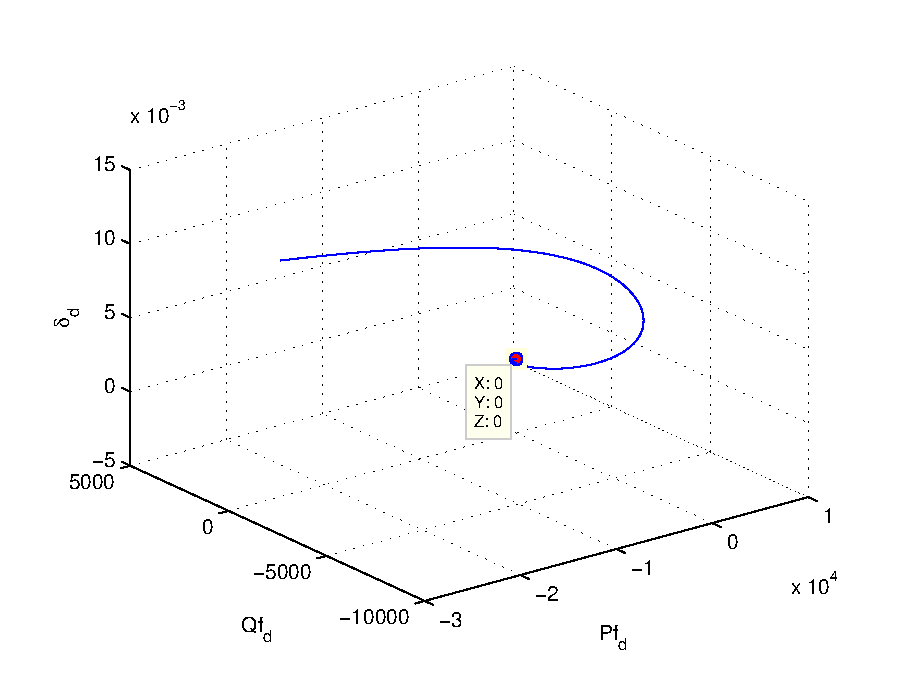
\includegraphics[width=10cm]{droop_answer_to_arbitrary_initial_value_var_desv}
	\caption{Trajetória da resposta do sistema droop para o ponto inicial $x_{d_{inicial}} = [-6252\quad1000\quad0.01]'$. A curva em azul corresponde á trajetória da resposta, enquanto o ponto em vermelho equivale ao ponto de equilíbrio do sistema}
	 \label{fig:resp_droop_var_desvio}
\end{figure}

Observe que o mesmo com o sistema redefinido para as varáveis de desvio, o comportamento do sistema continuou o mesmo, porém agora convergindo para a origem, a qual corresponde ao novo ponto de equilíbrio do sistema com variáveis de desvio.

\begin{example}
[Processo de quatro tanques] O processo de quatro tanques, foi introduzido por Johansson \cite{article:johansson:2000} e atualmente é utilizado como objeto de estudo em diversas universidades ao redor do mundo, pois permite o estudo de modelagem, linearização e projeto de controladores para sistema não linear multivariável \cite{article:roinila:2008}. A Figura \ref{fig:processo4tanques} traz uma representação do processo de quatro tanques.

\begin{figure}[htbp]
	\centering
	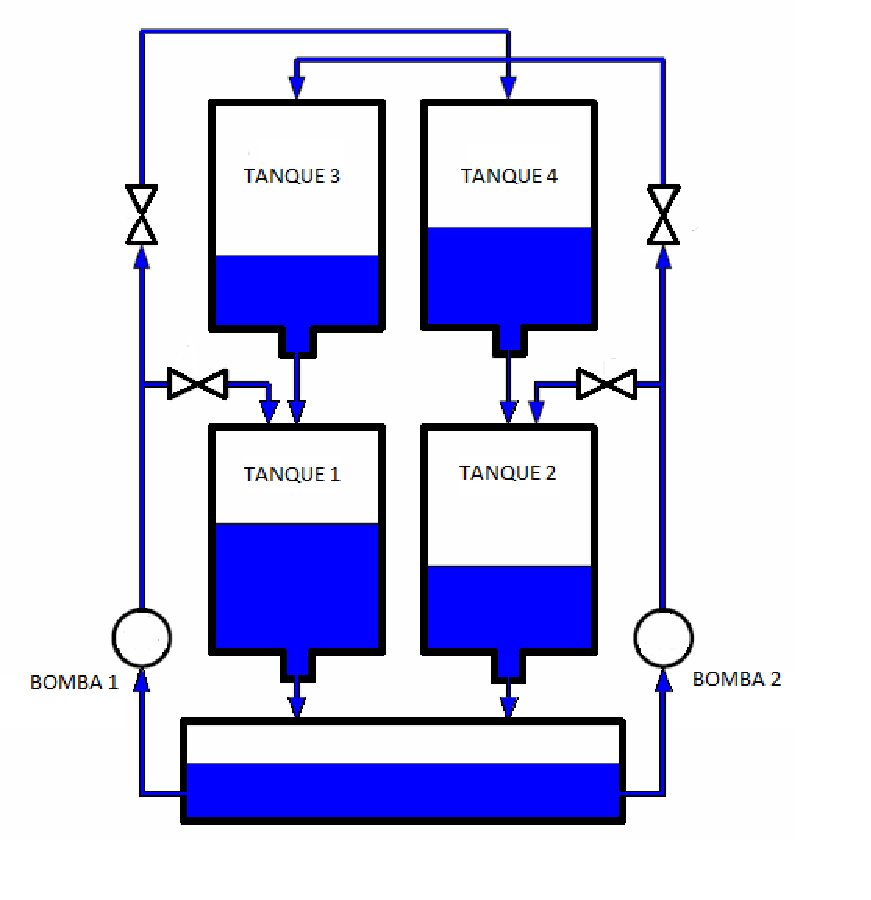
\includegraphics[width=8cm, height = 8cm]{4tanks}
	\caption{Diagrama esquemático do processo de quatro tanques}
	 \label{fig:processo4tanques}
\end{figure}

O objetivo deste processo é controlar os níveis dos tanques inferiores, tanques 1 e 2, utilizando-se as bombas 1 e 2. Assim, as entradas do processo são as tensões de entrada das bombas 1 e 2, que serão chamadas de $\upsilon_1$ e $\upsilon_2$, respectivamente. Já as saídas correspondem às tensões de medição dos níveis dos tanques 1 e 2. A partir destas tensões, é possível obter os níveis dos tanques propriamente ditos. Assim, as saídas correspondem ao nível $h_1$ do tanque 1 e ao nível $h_2$ do tanque 2.

A dinâmica deste processo é dita multivariável, pois cada uma das bombas afeta ambos os níveis $h_1$ e $h_2$ dos tanques 1 e 2. O acionamento da bomba 1 faz com que os tanques 1 e 4 sejam abastecidos e o tanque 4, por sua vez, despeja o líquido no tanque 2. De forma análoga, a bomba 2 abastece os tanques 2 e 3 e o tanque 3 despeja líquido no tanque 1.
A porcentagem do fluxo de líquido que vai para cada tanque está diretamente relacionada com a abertura das válvulas anteriores a estes. Esta proporção, ou taxa de líquido desviado para o tanque $i$, em que $i = 1, 2, 3, 4$, será representada pelo símbolo $\gamma_i$. Assim, a taxa de líquido desviado para o tanque $1$ será $\gamma_1$ e assim sucessivamente. Além disso, o volume de líquido em cada tanque será representado por $V_i$.

Dito isto, para obter a modelagem matemática do sistema, será considerado que o líquido utilizado no processo é água e será utilizada a equação de Bernoulli para líquidos incompressíveis
\begin{equation}\label{eq:Bernoulli}
 \dfrac{\rho \cdot v_i^2}{2} + \rho  \cdot g  \cdot h_i + P = constante 
\end{equation}
onde $\rho$ é a massa específica da água, $v_i$ é a velocidade de escoamento da água no tanque $i$, $g$ é a aceleração da gravidade, $h_i$ é a altura do nível do tanque $i$ e $P$ é a pressão. Além disso, utiliza-se o princípio de conservação de massa
\begin{equation}\label{eq:cons_massa}
\dot{V}_i = A_i  \cdot \dot{h}_i = q_{in} - q_{out} 
\end{equation}
em que $\dot{V}_i$ é a variação do volume de água do i-ésimo tanque, $A_i$ é a área da seção transversal e $\dot{h}_i$ é a variação da altura do nível do tanque $i$ ao longo do tempo. $q_{in}$ e $q_{out}$ são, respectivamente, os fluxos de entrada e de saída de água no tanque.

Assumindo a velocidade de escoamento $v_i$ na superfície da água é nula e que a altura $h_i$ do nível de água no tanque $i$ na parte inferior de cada tanque é zero, tem-se a equação de Bernoulli para a superfície da água tal que
\begin{equation}\label{eq:Bernoulli_sup}
 \rho  \cdot g  \cdot h_i + P = constante
\end{equation}

Já no fundo do tanque, a equação de Bernoulli será
\begin{equation}\label{eq:Bernoulli_fundo}
 \dfrac{\rho \cdot v_i^2}{2} + P = constante 
\end{equation}

Igualando as equações (\ref{eq:Bernoulli_sup}) e (\ref{eq:Bernoulli_fundo}), obtém-se a velocidade de escoamento da água
\begin{equation}\label{eq:vel_escoamento}
 v_i = \sqrt{g \cdot h_i} 
\end{equation}

O fluxo de saída do tanque é definido como o produto da velocidade de escoamento da água pela área da seção transversal $a_i$ da saída do tanque $i$. Já o fluxo de entrada se relaciona diretamente com o ganho de cada bomba e as tensões de entrada aplicadas \cite{inproc:arthur:2015}. Portanto as equações que regem o funcionamento do sistema são apresentadas as seguir, onde $\dot{h}_i$ é a variação da altura do tanque $i$ , $h_i$ é a altura do tanque $i$ e  $\upsilon_i$ é a tensão de entrada na bomba $i$ em um determinado instante de tempo, $ i = 1, 2, 3, 4$ e $j = 1, 2$.

\begin{equation*}
\begin{bmatrix}\dot{h_1}\\\dot{h_2}\\\dot{h_3}\\\dot{h_4}\end{bmatrix} = 
\begin{bmatrix}-\dfrac{a_1}{A_1}\cdot \dfrac{\sqrt{2\cdot g \cdot h_1}}{h_1}&0
&\dfrac{a_3}{A_1}\cdot \dfrac{\sqrt{2\cdot g \cdot h_3}}{h_3}&0
\\0&-\dfrac{a_2}{A_2}\cdot \dfrac{\sqrt{2\cdot g \cdot h_2}}{h_2}
&0&\dfrac{a_4}{A_2}\cdot \dfrac{\sqrt{2\cdot g \cdot h_4}}{h_4}
\\0&0&-\dfrac{a_3}{A_3}\cdot \dfrac{\sqrt{2\cdot g \cdot h_3}}{h_3}&0
\\0&0&0&-\dfrac{a_4}{A_4}\cdot \dfrac{\sqrt{2\cdot g \cdot h_4}}{h_4}\end{bmatrix}
\begin{bmatrix}h_1\\h_2\\h_3\\h_4\end{bmatrix}+\end{equation*}
\begin{equation}\label{eq:4tanques_matrix}
\begin{bmatrix}\dfrac{\gamma_1}{A_1}k_1&0\\0&\dfrac{\gamma_2}{A_2}k_2
\\0&\dfrac{1 - \gamma_2}{A_3}k_2\\\dfrac{1 - \gamma_1}{A_4}k_1\end{bmatrix}
\begin{bmatrix}\upsilon_1\\\upsilon_2\end{bmatrix}
\end{equation}

Como restrição física da planta disponibilizada no laboratório, a altura do volume de água em cada um dos tanques é limitada na região contida por $[0, 23 cm]$, de forma que quando o tanque estiver totalmente cheio, a altura do volume de água será de $23 cm$. As áreas da seção transversal é igual para todos os tanques e equivale a $A_i = 47.6 cm^2$. Os ganhos $k_1$ e $k_2$ das bombas são, respectivamente, 8.63 e 12.72, cuja unidade física é $cm^2/ V \cdot s$. Considerou-se a aceleração da gravidade como sendo $978 cm/s^2$. As áreas das seções transversais de saída dos tanques em $cm^2$ equivalem a $a_1 = 0.071$, $a_2 = 0.057$, $a_3 = 0.071$ e $a_4 = 0.057$.
\label{example_4tanques}
\end{example}

Para este exemplo, assumiremos que as entradas terão valor unitário, ou seja, $\begin{bmatrix}\upsilon_1&\upsilon_2\end{bmatrix}' = \begin{bmatrix}1&1\end{bmatrix}'$. Será assumido também que a altura estacionária dos níveis dos tanques será $ h^* = \begin{bmatrix}8.9\quad&9.97\quad&8.65\quad&9.67\quad\end{bmatrix}' cm$ \cite{inproc:arthur:2015}.Como este sistema possui quatro variáveis de estado, a representação do retrato de fase não é possível.

\section{Modelagem fuzzy}\label{Modelo-fuzzy}

Lógica fuzzy \cite{techreport:seatle}, ou lógica nebulosa, é um conceito que surgiu com uma forma de processar dados, possibilitando a associação de conjuntos parciais, ou seja, de conjuntos que têm uma determinada faixa de probabilidade de aderir a um conceito esperado. Definida originalmente na literatura por Lotfi A. Zadeh \cite{article:zadeh:1990}, a lógica fuzzy permite tratar sistemas nebulosos de forma quantitativa. Esta abordagem consiste em obter os graus de associação de cada elemento $\mathbf{x}$ na configuração fuzzy, atribuídos por uma função de associação $\mathbf{\alpha(x)}$, a qual corresponde a um valor definido em $\mathbf{x}$ e está contida no intervalo [0, 1].

Quanto maior o valor de $\mathbf{\alpha(x)}$, maior o grau de associação de $\mathbf{x}$ na configuração. Desta maneira, quando a função de associação de um elemento $\mathbf{x_i}$ num conjunto $\mathbf{U_i}$ for igual a 0 (zero), implica que o elemento é completamente "não" $\mathbf{U_i}$. Caso seja igual a 1 (um), implica que o elemento $\mathbf{x_i}$ é completamente $\mathbf{U_i}$. Uma regra básica para a modelagem fuzzy e que garante coerência entre o modelo fuzzy e o modelo real é que o somatório de todas as funções de associação do modelo deve ser igual a 1 (um).

Um dado sistema variante no tempo com entradas $\mathbf{u(t)}$, respostas $\mathbf{y(t)}$ e estados $\mathbf{x(t)}$ é dito um sistema fuzzy \cite{article:zadeh:1990} se suas respectivas entradas, saídas ou estados ou, ainda, qualquer combinação desdes variam conforme uma lógica fuzzy. Uma classe de sistemas que são aproximadamente equivalentes a um dado sistema é uma classe de sistema fuzzy.

Sistemas fuzzy podem aparentar semelhança com sistemas estocásticos. Todavia, a fonte das incertezas não é estatística, mas tem a ver com a variação dos limites das funções de associação de entrada para as descrições de entradas, saídas ou estados. Assim, enquanto incertezas em sistemas estocásticos seguem a lógica convencional, sendo definidas apenas em termos binários - 0 (zero) ou 1 (um) -, as incertezas fuzzy podem variar quanto ao grau de associação a um determinado conjunto. De forma que, $\mathbf{x_i}$ pode ser uma pertinência de  $\mathbf{\alpha_i(x_i) = 0.5}$ ou $\mathbf{\alpha_i(x_i) = 0.27}$ em relação a um conjunto $\mathbf{U_i}$, por exemplo. Estes dois tipos de sistema, porém, são altamente complexos matematicamente e difíceis de analisar. Com os avanços tecnológicos das últimas décadas, computadores com alto processamento permitem o estudo de sistemas fuzzy com maior facilidade.

Uma característica importante de sistemas fuzzy a ser considerada neste trabalho é a convexidade \cite{article:zadeh:1990}. Uma configuração fuzzy é dita convexa se, e somente, se qualquer ponto de uma reta traçada entre dois pontos $\mathbf{x_1}$, menor que $\mathbf{\alpha(x_1)}$, e $\mathbf{x_2}$, menor que $\mathbf{\alpha(x_2)}$, for sempre menor que a função de associação para aquele ponto.

A utilização de lógica fuzzy provê uma maneira simples e direta de decompor um sistema não linear em sistemas lineares locais, fáceis de manipular, e também permite agrupar estes sistemas lineares locais para gerar um modelo completo de comportamento equivalente ao sistema não linear.

\subsection{Modelos fuzzy Takagi-Sugeno}\label{Modelo-fuzzy-TS}

A modelagem de sistemas que utilizam a lógica fuzzy conforme proposto por Takagi e Sugeno \cite{booktw:2003} - modelagem fuzzy Takagi-Sugeno -, permite obter os modelos lineares locais, ou regras modelo, de relações entre entrada e saída do sistema não linear utilizando regras fuzzy do tipo SE-ENT\~{A}O. Assim, o modelo fuzzy Takagi-Sugeno consiste na combinação de cada um dos modelos lineares gerados por cada regra
Estas regras são obtidas conforme descrito a seguir.

\textbf{SE} $\mathbf{ z_1(t)}$ é $\mathbf{M_{i1}}$ e ... e $\mathbf{ z_p(t)}$ é $\mathbf{M_{ip}}$

\begin{equation}\label{eq:fuzzy_TS_regras}
\textbf{ENT\~{A}O}  \begin{cases} \mathbf{\dot{x} = A}_i \mathbf{x}(t)\\\end{cases}, \quad \textrm{i = 1, 2, ..., r}
\end{equation}
Onde $\mathbf{M_{ij}}$ é o grau de associação, ou grau de pertinência, \textbf{r} é o número de regras do modelo, \textbf{x}(t) é o vetor de estados e $\mathbf{A_i}$ é um vértice do sistema. O vetor $\mathbf{z = [z_1(t), ..., z_p(t)]}$ é chamado de vetor de variáveis premissas do sistema fuzzy T-S e será assumido que  estes termos podem depender apenas das variáveis de estado e do tempo. Será considerado, sem perda de generalidade, que o modelo fuzzy Takagi-Sugeno (T-S) foi obtido a partir de um sistema não linear cujo ponto de equilíbrio é a origem, ou seja, $\textbf{x}^* = \textbf{0}$.

O número de regras do sistema fuzzy Takagi-Sugeno está diretamente relacionado com a quantidade \textbf{p} de variáveis de premissa, conforme a relação $\mathbf{r = 2^p}$.

\subsection{Modelagem por não linearidade de setor}\label{subsec:sector_nonlinearuty_modeling}

Não-linearidade de setor é uma metodologia de modelagem sistemática proposta por \cite{booktw:2003} utilizada para transformar sistemas não lineares em sistemas fuzzy Takagi-Sugeno \cite{articlets:1985}. Esta abordagem consiste na combinação convexa de modelos lineares variantes no tempo. Também conhecida como modelagem por vértices \cite{articlets:2009}, a modelagem por não linearidade de setor garante a transformação exata do sistema \cite{booktw:2003}, ou seja, o modelo fuzzy Takagi-Sugeno obtido é equivalente ao modelo não linear original. A principal vantagem desta modelagem, quando comparada com demais métodos, é a possibilidade do uso de ferramentas de programação semi-definidas, permitindo analisar o sistema e projetar controladores utilizando desigualdades matriciais lineares - LMIs.

A ideia central para a obtenção do modelo fuzzy Takagi-Sugeno via não linearidade de setor consiste na obtenção do setor global que contenha, para qualquer valor de $x(t)$, em que $x(t)$ é uma variável de estado do sistema, a função f(x(t)) correspondente ao modelo não linear, com $f(0) = 0$, tal que
\begin{equation}\label{eq:setor_global}
\dot{x} = f(x(t)) \in [a_1, a_2] x(t)
\end{equation}
Ou seja, deve-se obter uma região sobre o plano de estados na qual $f(x(t))$ sempre esteja contida. A Figura \ref{fig:setor_global} ilustra graficamente a configuração de um setor global para uma dada $f(x(t))$.

\begin{figure}[htbp]
	\centering
	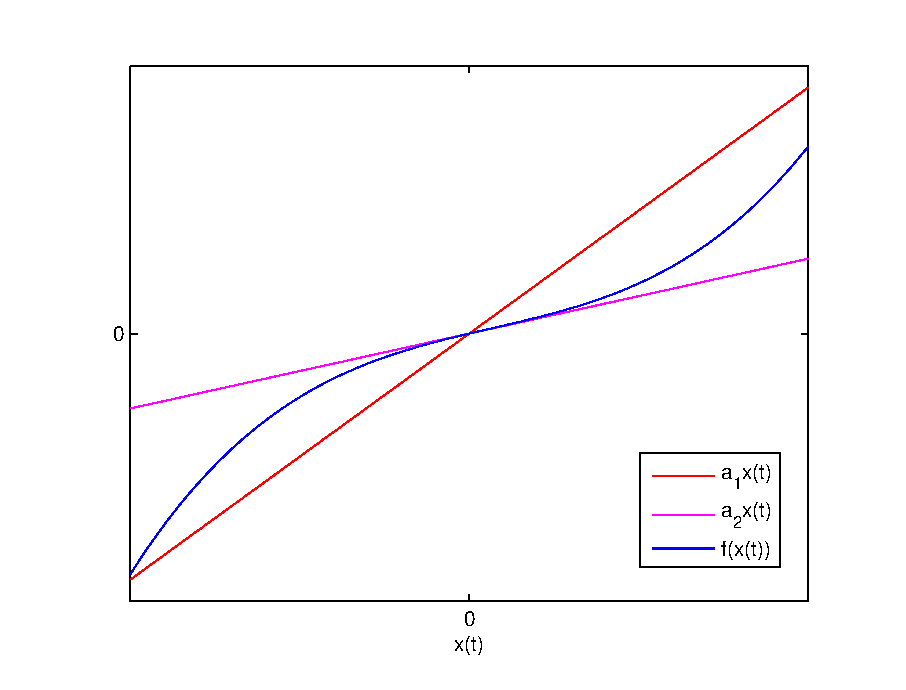
\includegraphics[width=10cm]{global_sector_nonlinearity}
	\caption{Setor global para um dado $f(x(t))$. As curvas em vermelho e em rosa correspondem às retas que limitam o setor global e a curva em azul equivale à função $f(x(t))$.}
	 \label{fig:setor_global}
\end{figure}

Nem sempre, porém, é possível prever o comportamento da função para quaisquer valores de $x(t)$, impossibilitando de se obter um setor global para a modelagem fuzzy Takagi-Sugeno exata do sistema. Assim, para sanar este problema, obtém-se o setor local, que consiste em um setor obtido da mesma forma que o setor global, porém limitado para valores pré-definidos de $x(t)$. A partir daí só se é possível garantir a exatidão do modelo dentro da região contida pelos limites de $x(t)$. Utilizam-se as restrições físicas das varáveis de estado do sistema como limitantes que definem a região do setor local. A Figura \ref{fig:setor_local} mostra a representação de um setor local, limitado por $-d \leq x(t) \leq d$.

\begin{figure}[htbp]
	\centering
	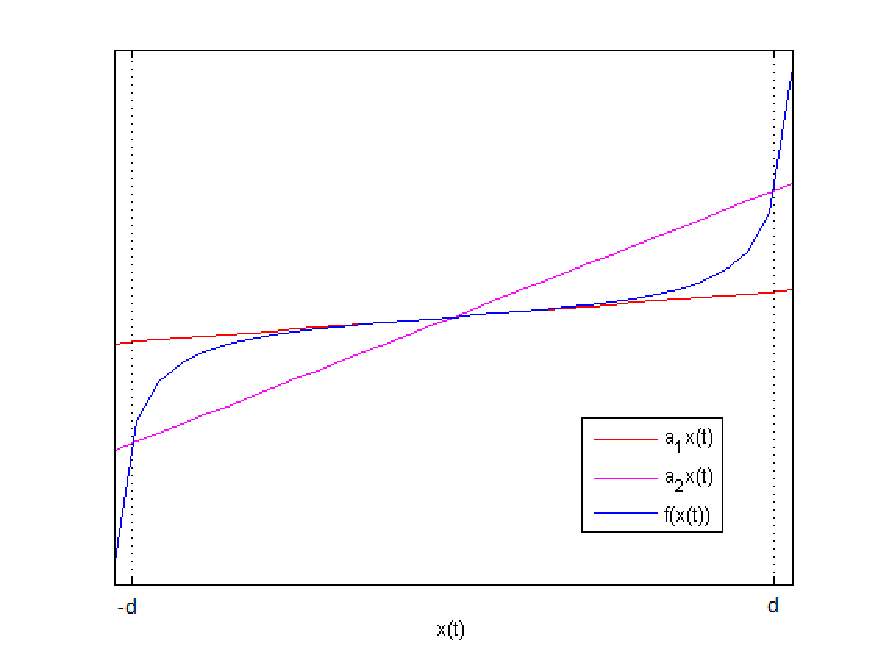
\includegraphics[width=10cm]{local_sector}
	\caption{Setor local para um dado $f(x(t))$. As curvas em vermelho e em rosa correspondem às retas que limitam o setor local e a curva em azul equivale à função $f(x(t))$. As linhas correspondentes aos limites de $x(t)$ estão representadas em preto pontilhado.}
	 \label{fig:setor_local}
\end{figure}

Assim, a modelagem fuzzy Takagi-Sugeno por não linearidade de setor local modela o sistema não linear de forma exata na região contida na configuração poliédrica $\chi$ definida em termos dos k vértices formados por todas as combinações dos limitantes das variáveis de estado, conforme segue.
\begin{equation}\label{eq:rep_poliedrica_por_vertices}
\mathbf{\chi} = co\{x^1, x^2, ... , x^k\}
\end{equation}

Como cada vértice $x^i, i = 1, 2, ..., k$, corresponde a uma combinação diferente entre cada um dos limites superiores e inferiores das variável de estado do sistema, então a região possuirá  $2^n$ vértices. Assim, se um sistema possui três variáveis de estado, por exemplo, haverá 8 vértices delimitando a região poliédrica que contém o ponto de equilíbrio e dentro da qual o sistema será modelado.

 Deste modo, para um sistema com duas variáveis de estado $x_1$ e $x_2$, por exemplo, tal que $-1 \leq x_1 \leq 1 $ e $-2 \leq x_2 \leq 2$, a modelagem por não linearidade de setor local permite obter um modelo válido dentro de uma região poliédrica descrita por quatro vértices resultantes das combinações dos pontos que limitam $x_1$ e $x_2$, os quais são $x^1 = (-1, -2), x^2 = (-1, 2), x^3 = (1, -2), x^4 = (1, 2)$. Esta região pode ser representada graficamente, conforme a Figura \ref{fig:poliedro_exemplo}.

\begin{figure}[htbp]
	\centering
	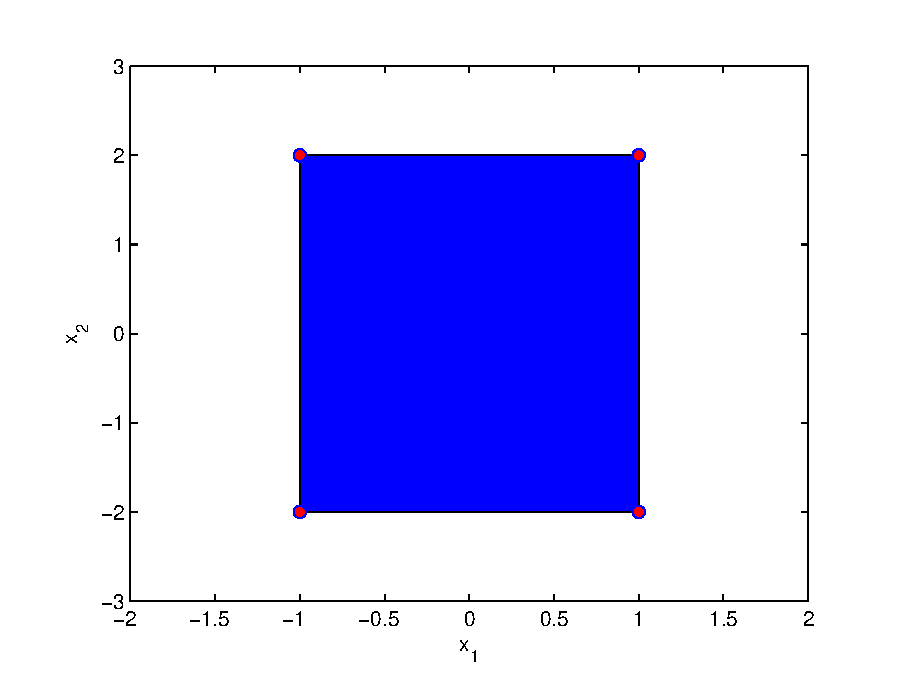
\includegraphics[width=10cm]{polyhedral_set_example}
	\caption{Região poliédrica $\chi$ de um sistema com variáveis de estado limitadas $-1 \leq x_1 \leq 1 $ e $-2 \leq x_2 \leq 2$, em que $\chi$ está representado em azul e os vértices correspondem aos pontos em vermelho.}
	 \label{fig:poliedro_exemplo}
\end{figure}

O modelo fuzzy Takagi-Sugeno obtido a partir do método de não linearidade por setor local apresenta, considerando um modelo não linear com a origem como ponto de equilíbrio, tal qual apresentado na equação \ref{eq:nonlinear_system_without_u}, a seguinte configuração
\begin{equation}\label{eq:fuzzyTS_system}
\mathbf{\dot{x}} = \mathbf{A(\alpha) x}
\end{equation}

Portanto, o objetivo desta o modelagem é obter $\mathbf{A(\alpha)}$, em que
\begin{equation}\label{eq:A_alpha}
\mathbf{A(\alpha)} = \sum_{i=1}^{r} \alpha_i(z) A_i,\qquad\alpha\in\Lambda_r
\end{equation}
Tal que
\begin{equation}\label{lambda_r}
\Lambda_r = \{\alpha \in \rm I\!R^r | \sum_{i = 1}^{r} \alpha_i(z) = 1,\quad \alpha_i(z) \geq 0\}
\end{equation}
De forma que $\alpha_i$ equivale à i-ésima função de associação e $A_i$ ao i-ésimo vértice do sistema, dados os limitantes físicos das variáveis de estado, e r é o número de regras fuzzy. O conjunto $\alpha_i$ das funções de associação é conhecido como primeiro simplex. Os parágrafos seguintes visam apresentar como se obter as funções de associação e os vértices do modelo fuzzy em estudo fazendo-se uso de um exemplo.

A partir a região $\chi$ de interesse e do sistema não linear o qual se pretende obter o modelo fuzzy Takagi-Sugeno, é preciso primeiramente identificar os termos não lineares do sistema, que corresponderão às variáveis de premissa $z_i(x(t)), i = 1, ..., n$ \footnote{A partir deste ponto o argumento t será omitido, para fins de simplificação da notação}. Assim, consideremos o exemplo a seguir retirado da \cite{articlets:2009}, que consiste em um sistema não linear simples que servirá como guia para o entendimento dos métodos de obtenção das fun\c{o}\~ {o}es de pertinência e dos vétices do modelo fuzzy.

\begin{example}
\begin{equation}\label{eq:ex_sal09}
 \begin{bmatrix}\dot{x_1}\\ \dot{x_2} \end{bmatrix} = \begin{bmatrix}0&1 \\-\sin(x_1^2)&0\end{bmatrix}\begin{bmatrix}x_1 \\x_2\end{bmatrix}, \chi = \{(x_1, x_2) | |x_1| \leq 0.5\}
\end{equation}\label{ex:sal09}
\end{example}

\'{E} possível verificar que há apenas uma variável de premissa, $z_1(x) = \sin(x_1^2)$. Conhecendo-se $\chi$, obtêm-se os limites superiores e inferiores de $z_1(x)$, os quais são, respectivamente, $min(z_1(x)) = z_1(0) = 0$ e $max(z_1(x)) = z_1(0.5) = 0.2474$. A não linearidade pode ser expressa, seguindo a metodologia de modelagem por não linearidade por setor local, com uma interpolação entre 0 e 0.2484 dependente do estado $x_1$, conforme a Figura \ref{fig:setor_local_ex_sal09}.
\begin{figure}[htbp]
	\centering
	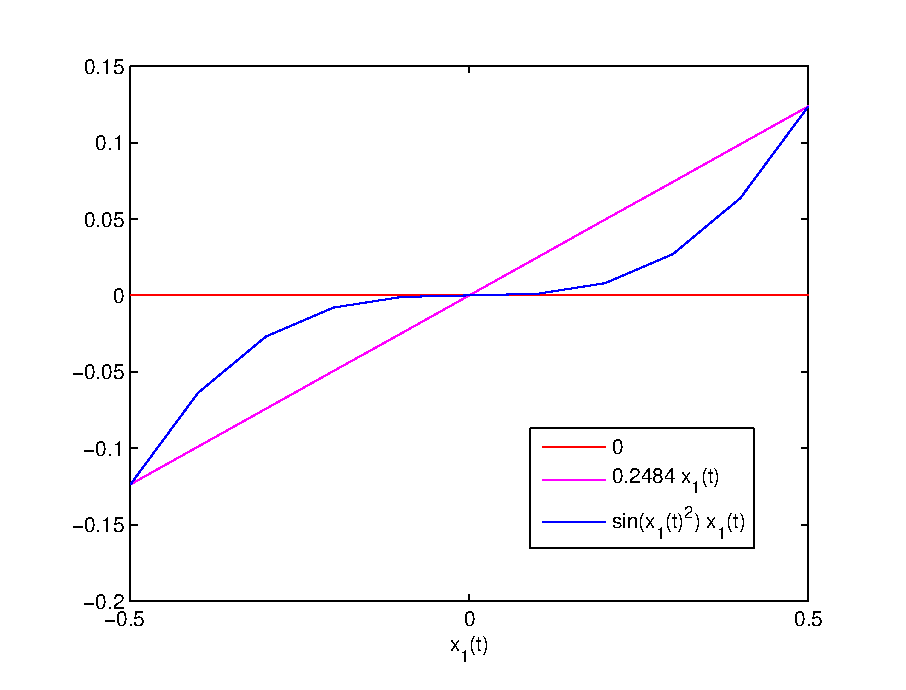
\includegraphics[width=10cm]{local_sector_ex_sal09}
	\caption{Setor local para a não linearidade $z_1 = \sin(x_1^2)$. A curva em vermelho corresponde ao limite inferior da não linearidade, a curva em rosa corresponde ao limite superior e a curva em azul equivale à própria  $z_1$}
	 \label{fig:setor_local_ex_sal09}
\end{figure}

Identificadas as variáveis de premissa e seus valores limites, estas podem ser representadas como \cite{booktw:2003}
\begin{equation}\label{eq:var_premissas_por_grau_pert}
z_i(\textbf{x}) = M_{i1}[z_i(\textbf{x})] \cdot min(z_i(\textbf{x})) + M_{i2}[z_i(\textbf{x})] \cdot max(z_i(\textbf{x})),	\qquad i = 1, .., n
\end{equation}

De forma que $M_{i1}[z_i(x)]$ e $M_{i2}[z_i(\textbf{x})]$ são os grau de associação, ou graus de pertinência, da variável de premissa $z_i(\textbf{x})$. Em outras palavras, $M_{i1}[z_i(\textbf{x})]$ expressa o quanto o limitante superior está associado ao valor assumido por $z_i(\textbf{x})$ para cada valor de \textbf{x} e $M_{i2}[z_i(\textbf{x})]$ expressa o quanto o seu limitante inferior está associado ao valor assumido por $z_i(\textbf{x})$ para cada valor de \textbf{x}. Portanto, deve-se restringir os graus de pertinência para que  sempre seja válida a relação \cite{booktw:2003}
\begin{equation}\label{eq:grau_pert_igual_1}
M_{i1}[z_i(\textbf{x})] + M_{i2}[z_i(\textbf{x})] = 1
\end{equation}

Além disso, $M_{ij}$ devem sempre estar contidos no intervalo [0, 1]. Quando o grau de associação for zero para algum valor de \textbf{x}, implica que $z_i(\textbf{x})$ é corresponde a exatamente o valor do limitante oposto ao deste grau de associação para este valor de \textbf{x}.

Por isso, os graus de associação podem ser calculados conforme mostra a equação \ref{eq:membership_degrees} \cite{booktw:2003}.
\begin{equation}\label{eq:membership_degrees}
M_{i1}[z_i(\textbf{x})] =\dfrac{z_i(\textbf{x})-min(z_i(\textbf{x}))}{max(z_i(\textbf{x}))-min(z_i(\textbf{x}))}, \quad M_{i2}[z_i(\textbf{x})] = 1 - M_{i1} =\dfrac{max(z_i(\textbf{x}))-z_i(\textbf{x})}{max(z_i(\textbf{x}))-min(z_i(\textbf{x}))} 
\end{equation}

Retomando o exempto da equação (\ref{eq:ex_sal09}), obtemos o graus de associação de $z_1(\textbf{x})$, com base no que fora descrito acima. Assim,
\begin{equation}\label{eq:membership_degrees_ex_sal09}
M_{11}[z_1(\textbf{x})] =\dfrac{\sin(x_1^2)}{\sin(0.5^2)}, \quad M_{12}[z_1(\textbf{x})] = 1 - M_{11} =\dfrac{\sin(0.5^2) - \sin(x_1^2)}{\sin(0.5^2)}
\end{equation}

A Figura \ref{fig:setor_local_ex_sal09} mostra as curvas dos graus de associação do sistema para os diferentes valores de $x_1(t)$.

\begin{figure}[htbp]
	\centering
	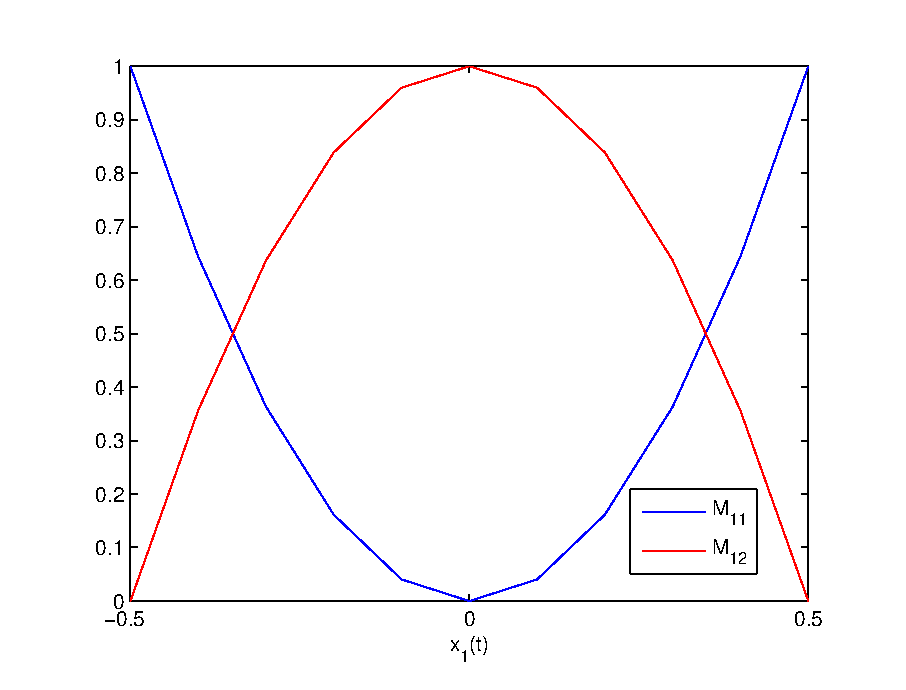
\includegraphics[width=10cm]{membershio_degrees_ex_sal09}
	\caption{Graus de pertinência de $z_1(\textbf{x})$ para o Exemplo \ref{ex:sal09}. A curva em azul corresponde a $M_{11}$ e a curva em vermelho corresponde a$M_{12}$}
	 \label{fig:setor_local_ex_sal09}
\end{figure}

As funções de associação ${\alpha[z(\textbf{x})]}$, por sua vez, relacionam os graus de pertinência das variáveis de premissa para obter o modelo de associação completo do sistema. Portanto, as funções de pertinência são obtidas conforme segue
\begin{equation}\label{eq:membership_functions}
\alpha_i (z)=\prod_{i_1 = 1}^{2} ... \prod_{i_n = 1}^{2} M_{1i_1}... M_{ni_n}
\end{equation}

Para o Exemplo \ref{ex:sal09}, como há apenas uma variável de premissa, as funções de associação equivalem aos graus de associação. Logo,
\begin{equation}\label{eq:membership_functions_ex_sal09}
\alpha_1(z) = \dfrac{\sin(x_1^2)}{\sin(0.5^2)}, \quad \alpha_2(z) = \dfrac{\sin(0.5^2) - \sin(x_1^2)}{\sin(0.5^2)}
\end{equation}

Por último, para se obter os vértices $\textbf{A}_i$ do modelo fuzzy Takagi-Sugeno, basta substituir todas variáveis de premissa $z_i(\textbf{x})$ na matriz $\textbf{A}$ do sistema não linear por cada uma das combinações  possíveis de seus valores máximos e mínimos \footnote{As combinações dos limitantes das variáveis de premissa em \textbf{A(x)} podem ser obtidas seguindo o modelo de representação binária sem sinal. Em que se assume que cada valor, iniciado por zero e indo até $2^n-1$, é representado por $n$ dígitos, sendo o primeiro correspondente a $z_1(\textbf{x})$ e o n-ésimo correspondente a $z_n(\textbf{x})$. Assim, quando o primeiro digito for 0 (zero),  $z_1(\textbf{x}) = min(z_1(\textbf{x}))$. Quando for 1 (um), $z_1(\textbf{x}) = max(z_1(\textbf{x}))$, e assim sucessivamente.}.

No exemplo que vimos nesta seção, os vértices são
\begin{equation*}
\textbf{A}_1 (\textbf{z}) =
 \begin{bmatrix}0&1 \\-min(z_1)&0\end{bmatrix} = 
\begin{bmatrix}0&1 \\-\sin(0)&0\end{bmatrix} = 
\begin{bmatrix}0&1 \\0&0\end{bmatrix}
\end{equation*}
\begin{equation*}
\textbf{A}_2(\textbf{z})= \begin{bmatrix}0&1 \\-max(z_1)&0\end{bmatrix} = \begin{bmatrix}0&1 \\-\sin(0.5^2)&0\end{bmatrix} = \begin{bmatrix}0&1 \\-0.2474&0\end{bmatrix}
\end{equation*}

\subsection{Algoritmo para obtenção do modelo fuzzy Takagi-Sugeno}

Com base no que fora dito até agora, é possível obter o modelo fuzzy Takagi-Sugeno para um setor local para qualquer sistema não linear seguindo os passos listados a seguir, tendo em mente que o sistema defuzificado será no formato

\begin{equation}\label{eq:modelo_fuzzy_TS}
\mathbf{\dot{x}} =\sum_{i=1}^{r}\alpha_i(z( \mathbf{x})) \mathbf{A_ix}
\end{equation}

\begin{enumerate}
\item Dado um sistema de equações não lineares com entradas forçadas nulas, representá-lo na forma matricial, tal que
\begin{equation*}
\mathbf{\dot{x}} = \mathbf{A(x)x}
\end{equation*}
\item Identificar as variáveis de premissa $z_1, ... z_n$, onde cada uma equivale a uma não linearidade distinta em \textbf{A(x)} dependente de  \textbf{x}.
\item Obter a quantidade de regras $r$ do modelo, a partir da quantidade $n$ de variáveis de premissa obtidas no item anterior, conforme segue.
\begin{equation*}
r = 2^n
\end{equation*}
\item A partir das limitações físicas das variáveis de estado do sistema, ou seja, a partir dos limites de valores que cada variável de estado pode assumir, definir os valores máximo, $max(z_i)$, e mínimo, $min(z_i)$, de cada variável de premissa.
\item Obter os graus de pertinência $M_{ij}$ do modelo para cada variável de premissa, conforme a Equação (\ref{eq:membership_degrees}).
\item Obter as $r$ funções de pertinência, conforme Equação (\ref{eq:membership_functions}).
\item Obter os $r$ vértices $\mathbf{A_i}$ do modelo, a partir da aplicação de todas as $2^n$ combinações possíveis dos valores máximos e mínimos das variáveis de premissa na matriz \textbf{A(x)} do modelo não linear.
\item Finalmente, utilizar os dados obtidos nos itens anteriores para montar o modelo defuzzificado da Equação (\ref{eq:modelo_fuzzy_TS}).
\end{enumerate}

\subsection{Exemplos}

Nesta seção serão apresentadas as modelagens fuzzy Takagi-Sugeno dos três exemplos apresentados na seção \ref{subsection:descr_exemplos}.

\begin{example}[Sistema não linear de segunda ordem \cite{article:LPJ:2011}]\end{example}\label{ex:LPJ12_fuzzyTS}
O exemplo \ref{example_LPJ12} consiste em um sistema de segunda ordem de dinâmica não linear, descrito conforme Equação (\ref{eq:LPJ12_dinamica}), em que $x_1$ é limitado por $-\pi/2 \leq x_1 \leq pi/2$

\begin{equation}\label{eq:LPJ12_dinamica}
\begin{bmatrix}\dot{x_1}\\ \dot{x_2} \end{bmatrix} = \begin{bmatrix} -2 & 4\\  -1 - \dfrac{\lambda (1 - sen(x_1))}{2} & -2 \end{bmatrix} \begin{bmatrix}x_1 \\ x_2 \end{bmatrix}
\end{equation}

Nota-se que o sistema possui apenas um termo não linear, ou seja, possui apenas uma variável de premissa $z_1 = sen(x_1(t))$. Conhecendo-se os limitantes da variável de estado $x_1$, obtemos os limitantes de $z_1$. Assim,

\begin{equation*}max(z_1(x(t))) = 1\quad min(z_1(x(t))) = -1\end{equation*}

Assim, obtém-se as funções de pertinência e os vértices do modelo fuzzy Takagi-Sugeno deste sistema, que são apresentados no Exemplo 2 da referência bibliográfica \cite{article:LPJ:2011}, conforme segue.
\begin{equation*}
\alpha_1(z(t)) = \dfrac{1+\sin(x_1(t))}{2}\qquad \alpha_2(z(t)) = 1 - h_1(z(t))
\end{equation*}
\begin{equation*}
A_1 = \begin{bmatrix}-2&4\\-1&-2\end{bmatrix}\qquad A_2 = \begin{bmatrix}-2&4\\-(1+\lambda)&-2\end{bmatrix}
\end{equation*}

O sistema não linear e o sistema fuzzy Takagi-Sugeno foram simulados e as curvas das respostas plotadas, conforme mostra a Figura \ref{fig:sim_fuzyy_TS_ex2_LPJ12}. Escolheu-se arbitrariamente o ponto inicial $\begin{bmatrix}x_{{inicial}_1}&x_{{inicial}_2}\end{bmatrix}' = \begin{bmatrix}-\pi/3&\pi/3\end{bmatrix}'$.

\begin{figure}[htbp]
	\centering
	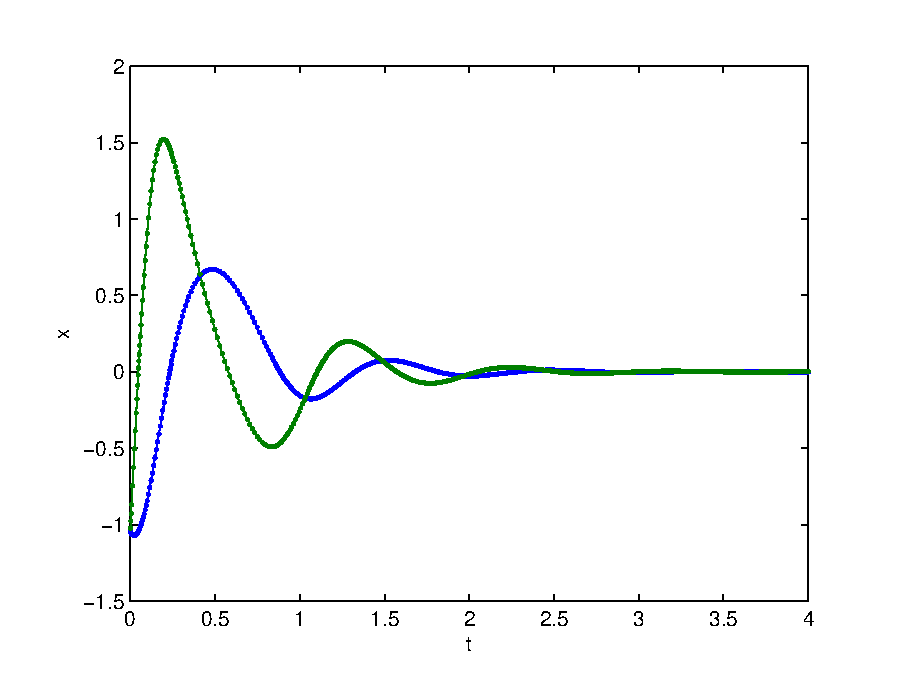
\includegraphics[width=10cm]{fuzzy_TS_sim_ex2_LPJ12}
	\caption{Respostas $x_1$ e $x_2$ do modelo não linear e do modelo fuzyy Takagi-Sugeno para o sistema de segunda ordem \cite{article:LPJ:2011}. As curvas em azul equivalem a $x_1$ e as curvas em verde a $x_2$. O modelo não linear corresponde às linhas contínuas, enquanto o modelo fuzzy T-S corresponde ás linhas pontilhadas}
	 \label{fig:sim_fuzyy_TS_ex2_LPJ12}
\end{figure}

As curvas obtidas da simulação dos modelos não linear e fuzzy T-S do exemplo \ref{ex:LPJ12_fuzzyTS} permitem verificar que estes modelos são completamente correspondentes entre si.

\begin{example}[Sitema droop]\label{ex:droop_UFSM_fuzzyTS}

Considerando o Exemplo \ref{ex:droop_UFSM}, que consiste no modelo Droop do inversor, as equações do sistema não linear com o ponto de equilíbrio na origem podem ser apresentadas na forma matricial, conforme segue.

\begin{equation}\label{eq:sist_droop_UFSM_mat}
\begin{bmatrix}\dot{x_{d_1}}\\\dot{x_2}\\\dot{x_3}\end{bmatrix} =\begin{bmatrix}-\omega_f - \dfrac{-\omega_fVn}{R_o}\cos(x_3)&0&\frac{\varphi(x_3)}{x_3}\\
\dfrac{\omega_fVn}{R_o}\sin(x_3)&-\omega_f&-\dfrac{\omega_fV(E_{ref}-n(x_1^*-P_{ref}))}{R_o}\dfrac{\sin(x_3)}{x_3}\\
0&m&0\end{bmatrix}\begin{bmatrix}x_{d_1}\\x_2\\x_3\end{bmatrix}
\end{equation}
onde $\varphi(x_3) = \dfrac{\omega_f}{R_o}(V(E_{ref}-n(x_1^* - P_{ref}))\cos(x_3) - V^2) - \omega_fx_1^*$.
\end{example}

O sistema possui quatro variáveis de premissa
\begin{equation*}
  \begin{gathered}
z_1 = \cos(x_3)\\
z_2 = \dfrac{\varphi(x_3)}{x_3}\\
z_3 = \sin(x_3)\\
z_4 = \dfrac{sin(x_3)}{x_3}
\end{gathered}
\end{equation*}

Desta maneira, a matriz $A(x)$ da equação \ref{eq:sist_droop_UFSM_mat} pode ser reescrita em função das variáveis de premissa.
\begin{equation}\label{eq:A_z}
A(z) = \begin{bmatrix}-\omega_f - \dfrac{-\omega_fVn}{R_o}z_1&0&z_2\\
\dfrac{\omega_fVn}{R_o}z_3&-\omega_f&-\dfrac{\omega_fV(E_{ref}-n(x_1^*-P_{ref}))}{R_o}z_4\\
0&m&0\end{bmatrix}
\end{equation}

Os limites máximo e mínimo das variáveis de premissa são obtidos levando em consideração os limites físicos de $x_3$, os quais só permitem valores contidos na região $\begin{bmatrix}-0.02&0.1\end{bmatrix}$. Assim, os limites superiores e inferiores de $\textbf{z}$ são obtidos, conforme as seguintes relações.
\begin{equation*}
\begin{gathered}
z_{1_{min}} = min(\cos(x_3)) \qquad  z_{4_{max}} = max(\cos(x_3))\\
z_{2_{min}} = min(\dfrac{\varphi(x_3)}{x_3}) \qquad  z_{2_{max}} = min(\dfrac{\varphi(x_3)}{x_3})\\
z_{3_{min}} = min(\sin(x_3)) \qquad  z_{3_{max}} = max(\sin(x_3))\\
z_{4_{min}} = min(\dfrac{sin(x_3)}{x_3}) \qquad z_{4_{max}} = max(\dfrac{sin(x_3)}{x_3})
\end{gathered}
\end{equation*}

O ponto $x_3 = 0$ não deve ser considerado para a obtenção dos limitantes de $\textbf{z}$ para que sejam evitadas indeterminações. Como foram identificadas quatro variáveis de premissa a partir do modelo não linear, o modelo fuzzy possuirá dezesseis vértices, os quais são representados pelas matrizes $A_i, i = 1, ... ,16$, em função das diferentes combinações de$ z_{j_{min}}$ e $z_{j_{max}}, j = 1, ..., 4$, conforme descrito abaixo.
\begin{equation}\label{eq:A_fuzzy_4_vertices}
\begin{gathered}
A_1 = A(z_{1_{min}}, z_{2_{min}}, z_{3_{min}}, z_{4_{min}})\\
A_2 = A(z_{1_{min}}, z_{2_{min}}, z_{3_{min}}, z_{4_{max}})\\
A_3 = A(z_{1_{min}}, z_{2_{min}}, z_{3_{max}}, z_{4_{min}})\\
A_4 = A(z_{1_{min}}, z_{2_{min}}, z_{3_{max}}, z_{4_{max}})\\
A_5 = A(z_{1_{min}}, z_{2_{max}}, z_{3_{min}}, z_{4_{min}})\\
A_6 = A(z_{1_{min}}, z_{2_{max}}, z_{3_{min}}, z_{4_{max}})\\
A_7 = A(z_{1_{min}}, z_{2_{max}}, z_{3_{max}}, z_{4_{min}})\\
A_8 = A(z_{1_{min}}, z_{2_{max}}, z_{3_{max}}, z_{4_{max}})\\
A_9 = A(z_{1_{max}}, z_{2_{min}}, z_{3_{min}}, z_{4_{min}})\\
A_{10} = A(z_{1_{max}}, z_{2_{min}}, z_{3_{min}}, z_{4_{max}})\\
A_{11} = A(z_{1_{max}}, z_{2_{min}}, z_{3_{max}}, z_{4_{min}})\\
A_{12} = A(z_{1_{max}}, z_{2_{min}}, z_{3_{max}}, z_{4_{max}})\\
A_{13} = A(z_{1_{max}}, z_{2_{max}}, z_{3_{min}}, z_{4_{min}})\\
A_{14} = A(z_{1_{max}}, z_{2_{max}}, z_{3_{min}}, z_{4_{max}})\\
A_{15} = A(z_{1_{max}}, z_{2_{max}}, z_{3_{max}}, z_{4_{min}})\\
A_{16} = A(z_{1_{max}}, z_{2_{max}}, z_{3_{max}}, z_{4_{max}})\\
\end{gathered}
\end{equation}

Cada variável de premissa possui dois graus de associação, concordante com a equação \ref{eq:membership_degrees}. Já as funções de associação são obtidas a partir da equação \ref{eq:membership_functions}.

Finalmente, conhecendo-se os valores numéricos dos parâmetros do sistema, obtém-se o modelo fuzzy Takagi-Sugeno do sistema droop. Tanto o modelo não linear quanto o modelo fuzzy T-S deste sistema foram simulados para o valor inicial igual a $\begin{bmatrix}10000&1000&0.01\end{bmatrix}$, o qual está dentro do hiperplano $C$ delimitado pelos valores máximos e mínimos que cada variável de estado pode assumir. As curvas obtidas da simulação foram plotadas e são apresentadas na Figura \ref{fig:sim_fuzyy_TS_droop_UFSM}, lembrando que $x_1 = P_f$, $x_2 = Q_f$ e $x_3 = \delta$.

\begin{figure}[htbp]
	\centering
	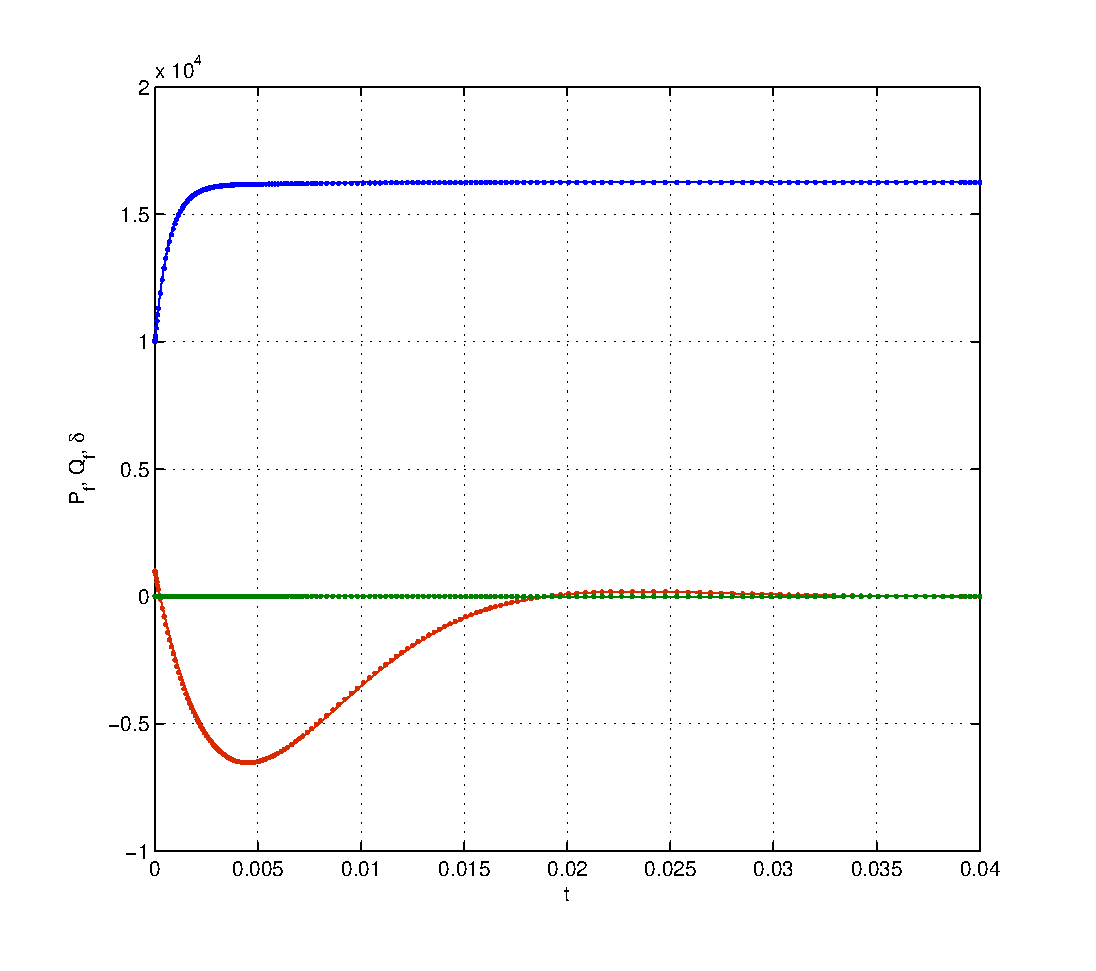
\includegraphics[width=10cm]{fuzzy_TS_sim_droop_UFSM}
	\caption{Respostas $P_f$, $Q_f$ e $\delta$ do modelo não linear e do modelo fuzzy Takagi-Sugeno para o sistema de droop com $\textbf{x}_{inicial} = [10000\quad1000\quad0]'$. As curvas em azul equivalem a $P_f$, as curvas em verde a $\delta$ e em vermelho, $Q_f$. O modelo não linear corresponde às linhas contínuas, enquanto o modelo fuzzy T-S corresponde às linhas pontilhadas}\label{fig:sim_fuzyy_TS_droop_UFSM}
\end{figure}

A Figura \ref{fig:sim_fuzyy_TS_droop_UFSM} evidencia que o modelo fuzzy T-S obtido corresponde a exatamente o modelo não linear do sistema.

Para verificar o comportamento dos estados fora do setor local delimitado por $C$, foi escolhido arbitrariamente um ponto $\textbf{x}_{inicial}$ fora desta região. O ponto escolhido foi $\textbf{x}_{inicial} = \begin{bmatrix}1000000&-100000&0.3\end{bmatrix}$' e as respostas do modelo não linear e do modelo fuzzy T-S são apresentadas na Figura \ref{fig:fuzzy_droop_out} e na Figura \ref{fig:sim_fuzzy_TS_droop_UFSM_out_of_C}.

\begin{figure}[htbp]
	\centering
	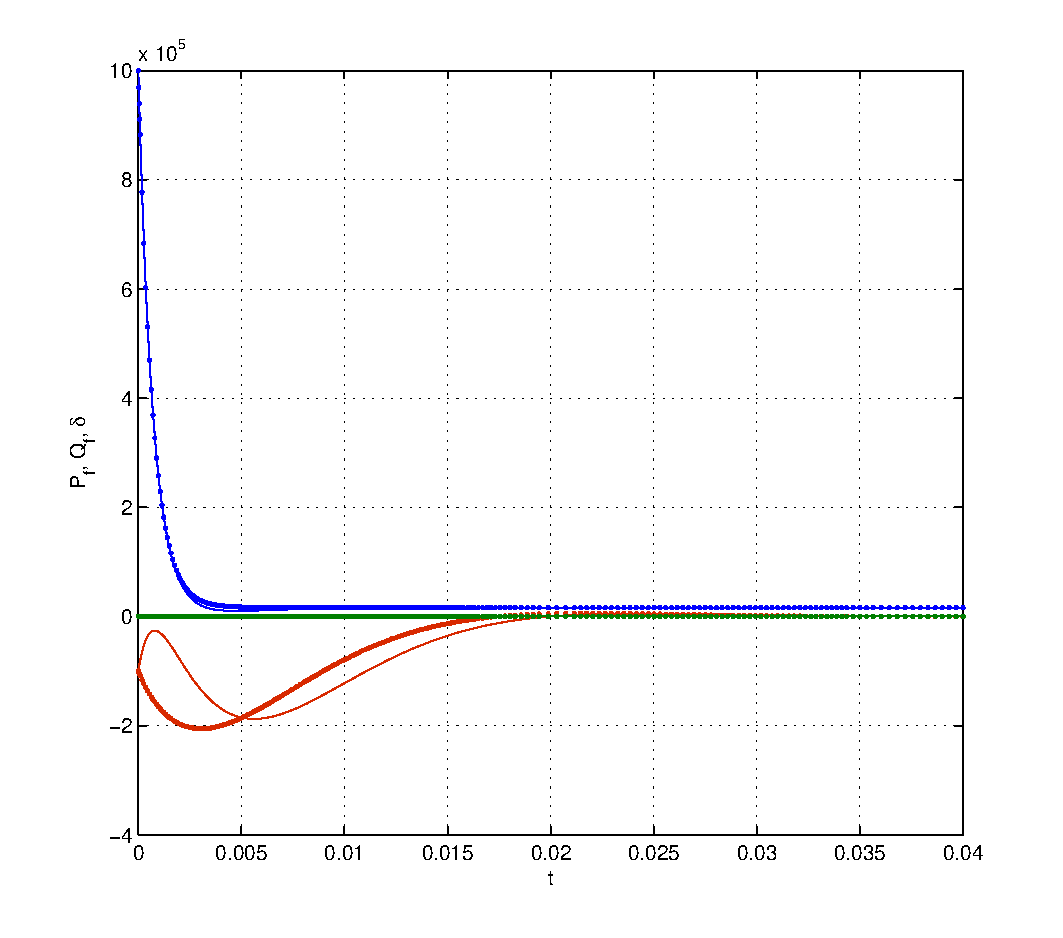
\includegraphics[width=10cm]{fuzzy_TS_sim_droop_UFSM_out_of_C}
	\caption{Respostas $P_f$, $Q_f$ e $\delta$ do modelo não linear e do modelo fuzyy Takagi-Sugeno para o sistema de droop com $\textbf{x}_{inicial} = [1000000\quad-100000\quad0.3]'$ fora da região $C$. As curvas em azul equivalem a $P_f$, as curvas em verde a $\delta$ e em vermelho, $Q_f$. O modelo não linear corresponde às linhas contínuas, enquanto o modelo fuzzy T-S corresponde às linhas pontilhadas}\label{fig:sim_fuzzy_TS_droop_UFSM_out_of_C}
\end{figure}

\begin{figure}[htbp]
	\centering
	\subfigure[ref1][$P_f$]{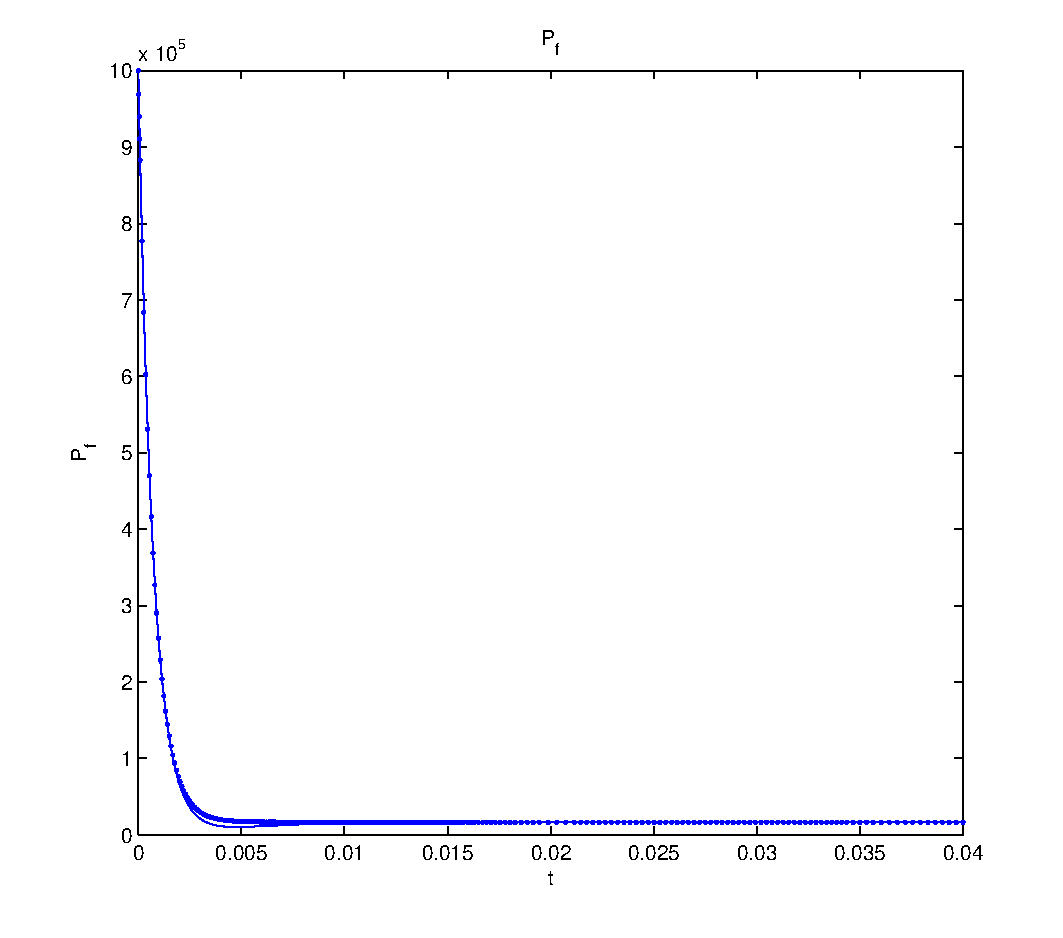
\includegraphics[width=7cm]{P_f_out_of_C}}
	\qquad
	\subfigure[ref2][$Q_f$]{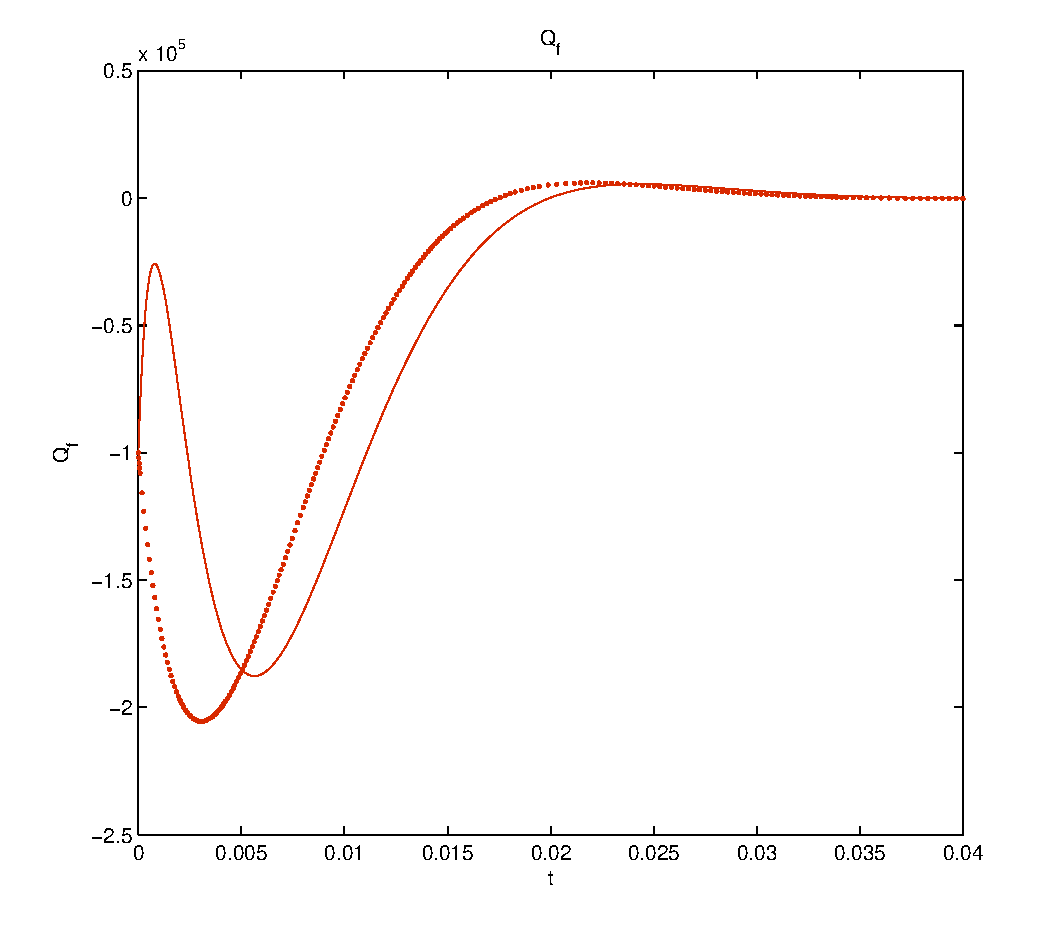
\includegraphics[width=7cm]{Q_f_out_of_C}}
	\qquad
	\subfigure[ref3][$\delta$]{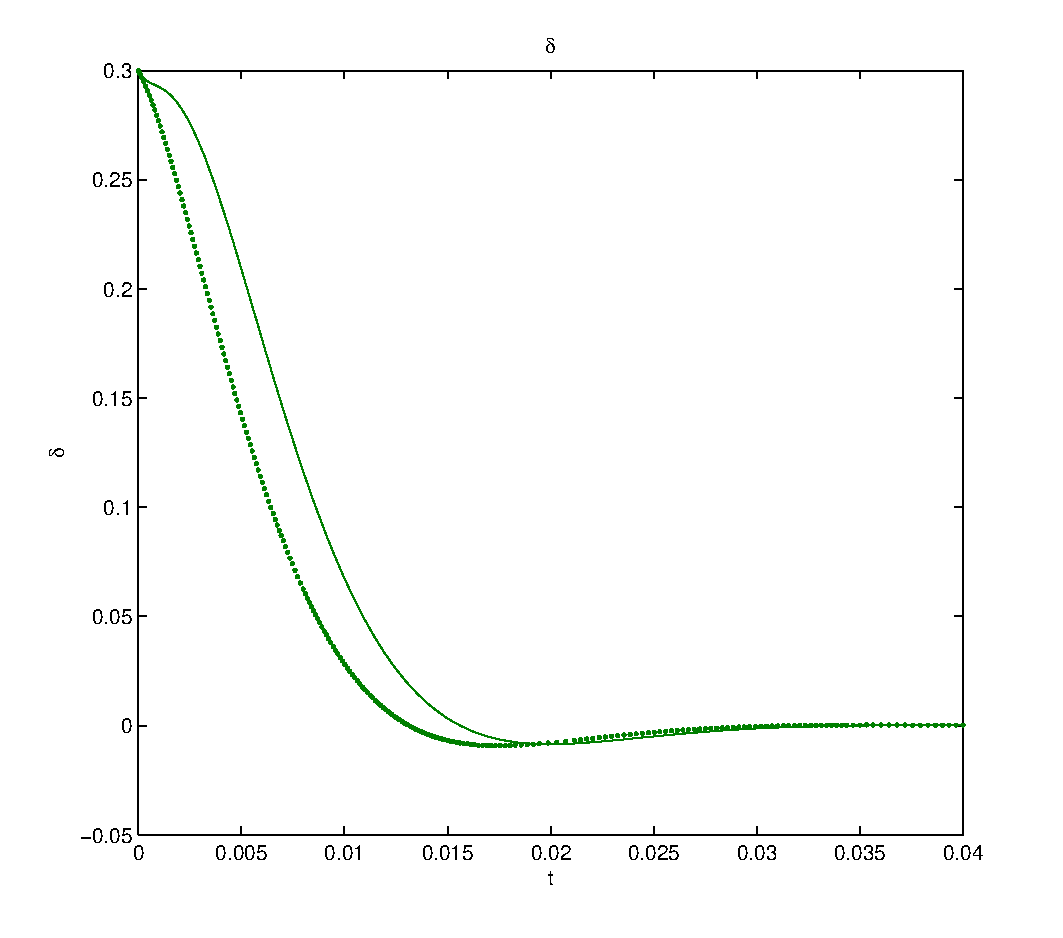
\includegraphics[width=7cm]{delta_out_of_C}}
	\caption{Resposta do sistema droop para o ponto inicial $\textbf{x}_{inicial} = [1000000\quad-100000\quad0.3]'$ fora da região $C$ em função do tempo. Em linha contínua são representadas as respostas dos modelo nã-linear e em pontilhado as respostas do modelo fuzzy}
	\label{fig:fuzzy_droop_out}
\end{figure}

A partir das Figuras \ref{fig:fuzzy_droop_out} e \ref{fig:sim_fuzzy_TS_droop_UFSM_out_of_C} é possível notar que o modelo fuzzy T-S não é válido fora da região C, para qual se obteve este modelo. Este conclusão é verificada pelo fato de que o modelo fuzzy T-S não corresponde ao modelo não linear para o ponto inicial fora de C.

\begin{example}[Processo de quatro tanques]\label{ex:4_tanques} O exemplo \ref{example_4tanques} apresenta um sistema que utiliza duas bombas para controlar o nível de água dentro de dois tanques inferiores. Cada uma das bombas, além de abastecer um dos tanques inferiores, também abastece um dos tanques superiores, os quais, por sua vez, despejam seus conteúdos nos tanques inferiores. O modelo não linear deste sistema é apresentado na forma matricial na Equação (\ref{eq:4tanques_matrix}). Além disso, devido ás limitações físicas da planta, foi assumido que as variáveis de estado $h_1$, $h_2$, $h_3$ e $h_4$ do sistema somente assumirão valores contidos no intervalo $[0, 23 cm]$.
\end{example}

A partir do modelo não linear, é possível verificar que o sistema possui quatro não linearidades, que serão equivalentes às variáveis de premissa do sistema, as quais são
\begin{equation*}
z_1 = \dfrac{\sqrt{(h_1)}}{h_1}\quad z_2 = \dfrac{\sqrt{(h_2)}}{h_2}\quad z_3 = \dfrac{\sqrt{(h_3)}}{h_3}\quad z_4 = \dfrac{\sqrt{(h_4)}}{h_4}
\end{equation*}

Os valores máximos $z_{i_{max}}$ e mínimos $z_{i_{min}}$ das variáveis de premissa são obtidos desconsiderando o ponto $h_i = 0$, para que não ocorra a indeterminação de divisão por zero. Desta maneira, obtiveram-se  $z_{i_{max}} = 3.1623$ e $z_{i_{min}} = 0.2085, i = 1, 2, 3, 4$.

Por ter quatro variáveis de premissa, o sistema possui dezesseis vértices. A matriz $\textbf{A(x)}$ do modelo não linear do processo pode ser reescrita em função das variáveis de premissa, conforme mostra a Equação (\ref{eq:A_z_fuzzy_4_tqs}).
\begin{equation}\label{eq:A_z_fuzzy_4_tqs}
\textbf{A(z)} =\begin{bmatrix}-\dfrac{a_1}{A_1}\cdot \sqrt{2\cdot g}\cdot z_1&0
&\dfrac{a_3}{A_1}\cdot \sqrt{2\cdot g}\cdot z_3&0
\\0&-\dfrac{a_2}{A_2}\cdot \sqrt{2\cdot g }\cdot z_2
&0&\dfrac{a_4}{A_2}\cdot \sqrt{2\cdot g}\cdot z_4
\\0&0&-\dfrac{a_3}{A_3}\cdot \sqrt{2\cdot g}\cdot z_3&0
\\0&0&0&-\dfrac{a_4}{A_4}\cdot \sqrt{2\cdot g }\cdot z_4\end{bmatrix}
\end{equation}

Os vértices de 16 $\textbf{A(z)}$ são obtidos a partir de todas as combinações possíveis entre dos valores máximos e mínimos das variáveis de premissa, conforme já apresentado na Equação (\ref{eq:A_fuzzy_4_vertices}).

Cada variável de premissa possui dois graus de associação, que são obtidos a partir da Equação (\ref{eq:membership_degrees}). As funções de associação, por sua vez, são obtidas a partir da Equação (\ref{eq:membership_functions}).

A matriz $B$, associada às entradas do sistema, também compõe os vértices do sistema. Porém, como $B$ não depende dos estados, continua no modelo fuzzy exatamente como é para o modelo não linear, de forma que os 16 vértices $B_i, i = 1, 2,\hdots, 16$ serão iguais a $B$.

Neste exemplo, o modelo defuzzyficado aparece na forma
\begin{equation}\label{eq:fuzzyTS_system_with_B}
\mathbf{\dot{x}} = \mathbf{A(\alpha)x+Bu}
\end{equation}
Que pode ser reescrita como
\begin{equation}\label{eq:A_alpha_B}
\mathbf{\dot{x}} = \sum_{i=1}^{r} \alpha_i(z) A_ix + Bu
\end{equation}

O modelo não linear e do modelo fuzzy Takagi-Sugeno do processo de quatro tanques foram simulados e as curvas de resposta foram obtidas, conforme mostra a Figura \ref{fig:4_tanques_sim_TS}. Embora o sistema tenha como limitação a altura máxima igual a $23 cm$ para o nível de água em cada um dos tanques, estas alturas não foram saturadas nas simulações. Isto foi feito para que se pudesse verificar a não exatidão do modelo fora da região da modelagem fuzzy Takagi-Sugeno.
\begin{figure}[htbp]
	\centering
	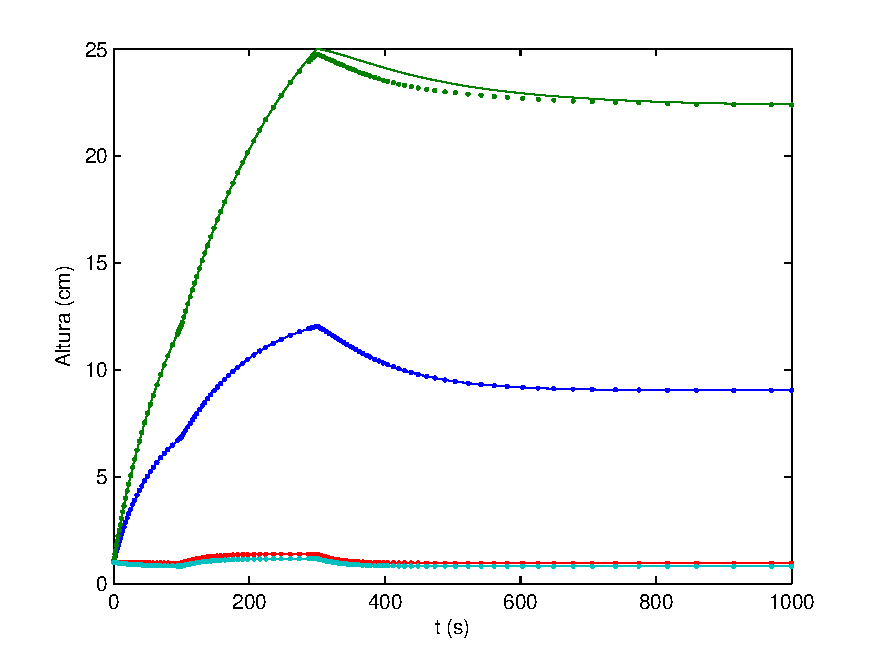
\includegraphics[width=10cm]{4_tanks_simulation}
	\caption{Respostas $h_1$, $h_2$, $h_3$ e $h_4$ do modelo não linear e do modelo fuzyy Takagi-Sugeno para o processo de quatro tanques com $\textbf{h}_{inicial} = [8.9\quad9.97\quad8.65\quad9.67]'$ e entradas $\upsilon = [1\quad1]$. As curvas em azul equivalem a $h_1$, em verde tem-se $h_2$, em vermelho, $h_3$, e em azul claro $h_4$. O modelo não linear corresponde às linhas contínuas, enquanto o modelo fuzzy T-S corresponde às linhas pontilhadas}\label{fig:4_tanques_sim_TS}
\end{figure}

A simulação do processo de quatro tanques permite concluir que a modelagem fuzzy Takagi-Sugeno modela de forma exata o sistema não linear dentro da região para a qual a modelo foi definido, ou seja, dentro do setor local. Em contrapartida, quando os estados se afastam da região para a qual o modelo fuzzy T-S foi definido, como é o caso de $h_1$, que ultrapassa a altura de $23 cm$ na simulação, é possível notar que o modelo deixa de ser exato.

\section{Considerações Finais}\label{sec:consid_finais}
Neste capítulo foi apresentado o conceito de retrato de fase para resposta de sistemas. O retrato de fase é utilizado para verificar de forma qualitativa a estabilidade do ponto de equilíbrio de sistemas não lineares, uma vez que estes têm um comportamento difícil de se prever, justamente devido aos termos não lineares que contêm. Vimos que quando as respostas se aproximam do ponto de equilíbrio à medida que o tempo passa, este é dito como estável. Por outro lado, quando as respostas se afastam do ponto de equilíbrio com o passar do tempo, diz-se que este ponto de equilíbrio é instável. Também foram vistos outros tipos de conclusões que podem ser verificadas a respeito da estabilidade de pontos de equilíbrio.
Os principais exemplos utilizados para aplicação dos conceitos discutidos neste trabalho também foram apresentados nesta seção. Por último, mas não menos importante, foi apresentada a técnica de modelagem por lógica fuzzy, proposta por Takagi e Sugeno \cite{articlets:1985} para a obtenção de um modelo constituído por um conjunto de representações linearizadas do sistema não linear. Este modelo garante a exatidão, quando comparado com o sistema não linear, dentro de uma região definida no plano de estados.

Para se obter o sistema fuzzy Takagi-Sugeno exato para uma região definida no espaço de estados, utilizou-se o artifício de modelagem por não linearidade de setor, proposto por Tanaka e Wang \cite{booktw:2003}. Os modelos fuzzy Takagi-Sugeno foram obtidos para cada um dos exemplos propostos e foi possível verificar a exatidão desta modelagem em relação ao modelo não linear para a região definida na obtenção do modelo. O contrário também foi observado quando para pontos fora da região para a qual o sistema fuzzy T-S foi obtido.

Nos próximos capítulos serão apresentadas técnicas para a análise de estabilidade de pontos de equilíbrio de sistemas utilizando o modelo fuzzy Takagi-Sugeno e função de Lyapunov, assim como técnicas para a obtenção do domínio de atração destes pontos de equilíbrio, quando estáveis. Os resultados obtidos neste capítulo serão utilizados tanto para obtenção das funções de Lyapunov para verificação da estabilidade, a partir do modelo fuzzy T-S, quanto para verificação de validade dos domínios de atração dos pontos de equilíbrio estável por meio de comparações com os respectivos retratos de fase.